The data and standard model MC samples used in this analysis are the same 
as in the SM Higgs search~\cite{HWWHCP2012}.
The additional signal samples for $gg\to X\to WW$,
were generated by using
JHUGen~\cite{JHUGen}, with the matrix elements
calculated at LO. The generated LHE files were
interfaced to PYTHIA for showering, hadronization, and the underlying event.
To validate the JHUGen $gg\to X\to WW$ event samples, we also produced 
standard model Higgs boson event samples by using JHUGen.  
These samples are described in Table~\ref{tab:DatasetsMC}. 
The method and results of the validation of JHUGen
are described in Section~\ref{sec:JHUGenval}.

%%%%%%%%%%%%%%%%%%%%%%%%%%%%%%%%%%%%%%%%%%%%%
\begin{table}[!ht]
\begin{center}
{\footnotesize
\begin{tabular}{|c|c|}
\hline
\multicolumn{2}{|c|}{With Pileup: Processed dataset name is always} \\
\multicolumn{2}{|c|}{/Summer12\_DR53X-PU\_S10\_START53\_V7A-v*/AODSIM} \\ 
\hline
 Dataset Description              		&   Primary Dataset Name  \\ 
\hline
$gg\to H\to WW\to (l\nu)(l\nu)$, $l=e,\mu$      & SMHiggsToWWTo2L2Nu\_M-125\_8TeV-jhu-pythia6 \\ 
$gg\to H\to WW\to (l\nu)(\tau\nu)$, $l=e,\mu$   & SMHiggsToWWToLTau2Nu\_M-125\_8TeV-jhu-pythia6 \\
$gg\to H\to WW\to (\tau\nu)(\tau\nu)$           & SMHiggsToWWToTauTau2Nu\_M-125\_8TeV-jhu-pythia6 \\
$gg\to \text{Graviton}\to WW\to (l\nu)(l\nu)$, $l=e,\mu$      & Graviton2PMToWWTo2L2Nu\_M-125\_8TeV-jhu-pythia6 \\ 
$gg\to \text{Graviton}\to WW\to (l\nu)(\tau\nu)$, $l=e,\mu$   & Graviton2PMToWWToLTau2Nu\_M-125\_8TeV-jhu-pythia6 \\
$gg\to \text{Graviton}\to WW\to (\tau\nu)(\tau\nu)$           & Graviton2PMToWWToTauTau2Nu\_M-125\_8TeV-jhu-pythia6 \\
\hline
\end{tabular}
}
\label{tab:DatasetsMC}
\caption{Summary of additional Monte Carlo datasets used at $\sqrt{s} = 8~\TeV$. 
Other samples are described in detail in~\cite{HWWHCP2012}. The same set of 
corresponding samples at $\sqrt{s} = 7~\TeV$ are also available and used in this study.}
\end{center}
\end{table}
%%%%%%%%%%%%%%%%%%%%%%%%%%%%%%%%%%%%%%%%%%%%%

\subsection{JHUGen validation}
\label{sec:JHUGenval}

To validate JHUGen, we compared the main kinematic distributions between JHUGen and
MCFM at the generator level, and to the Powheg-Pythia samples used in the
SM Higgs search at the reconstruction level.

Figure~\ref{fig:jhuvsmcfm} compares the main kinematic observables at generator 
level between the JHUGen and MCFM for events without any cuts. 
Both samples are generated with the Higgs boson produced at rest. 
We observe good agreement within a few percent in the bulk of the two distributions. 

%%%%%%%%%%%%%%%%%%%%%%%%%%%%%%%%%%%%%%%%%%%%%
\begin{figure}[!hbtp]
\centering
\subfigure[Leading Lepton $\pt$]{
\centering
\label{subfig:leadleppt}
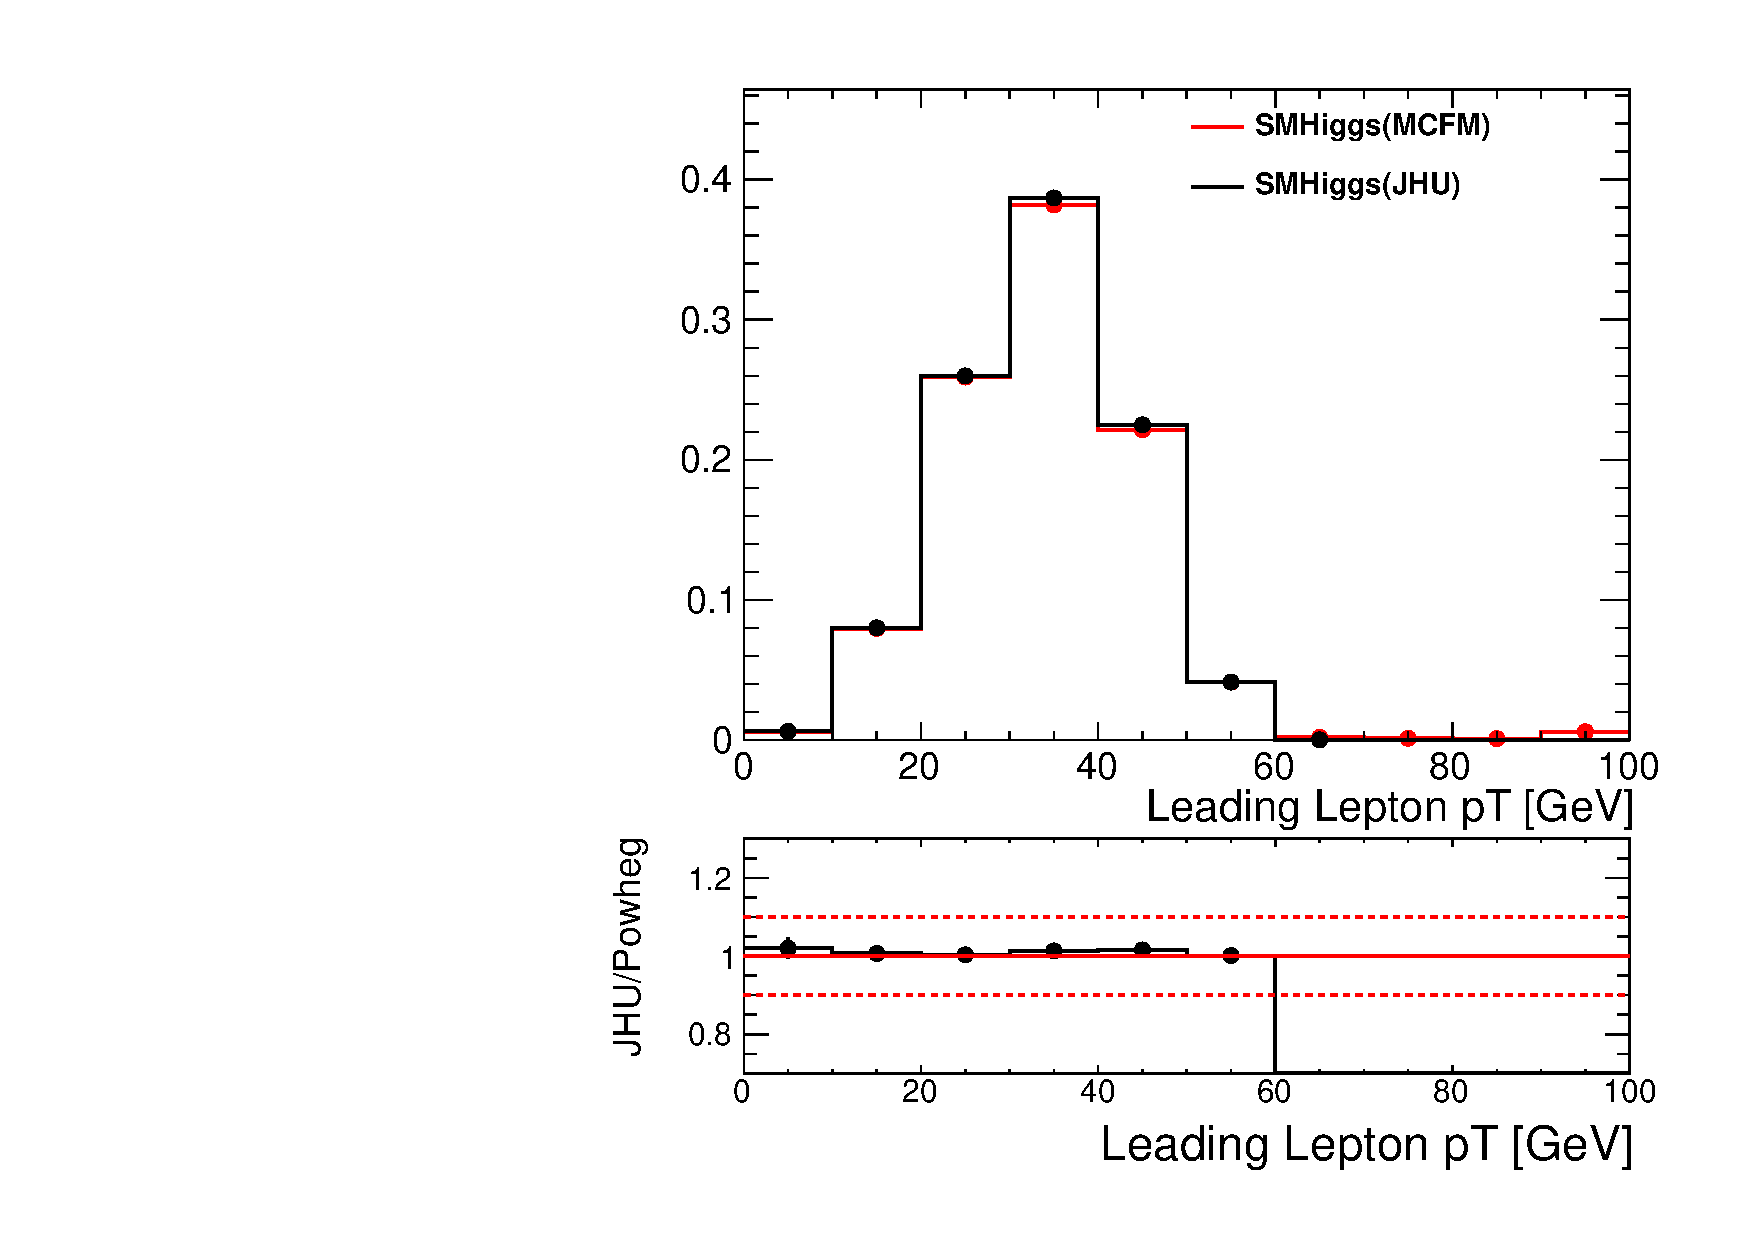
\includegraphics[width=.3\textwidth]{figures/leadleppt_jhuvsmcfm.pdf}
}
\subfigure[Trailing Lepton $\pt$]{
\centering
\label{subfig:trailleppt}
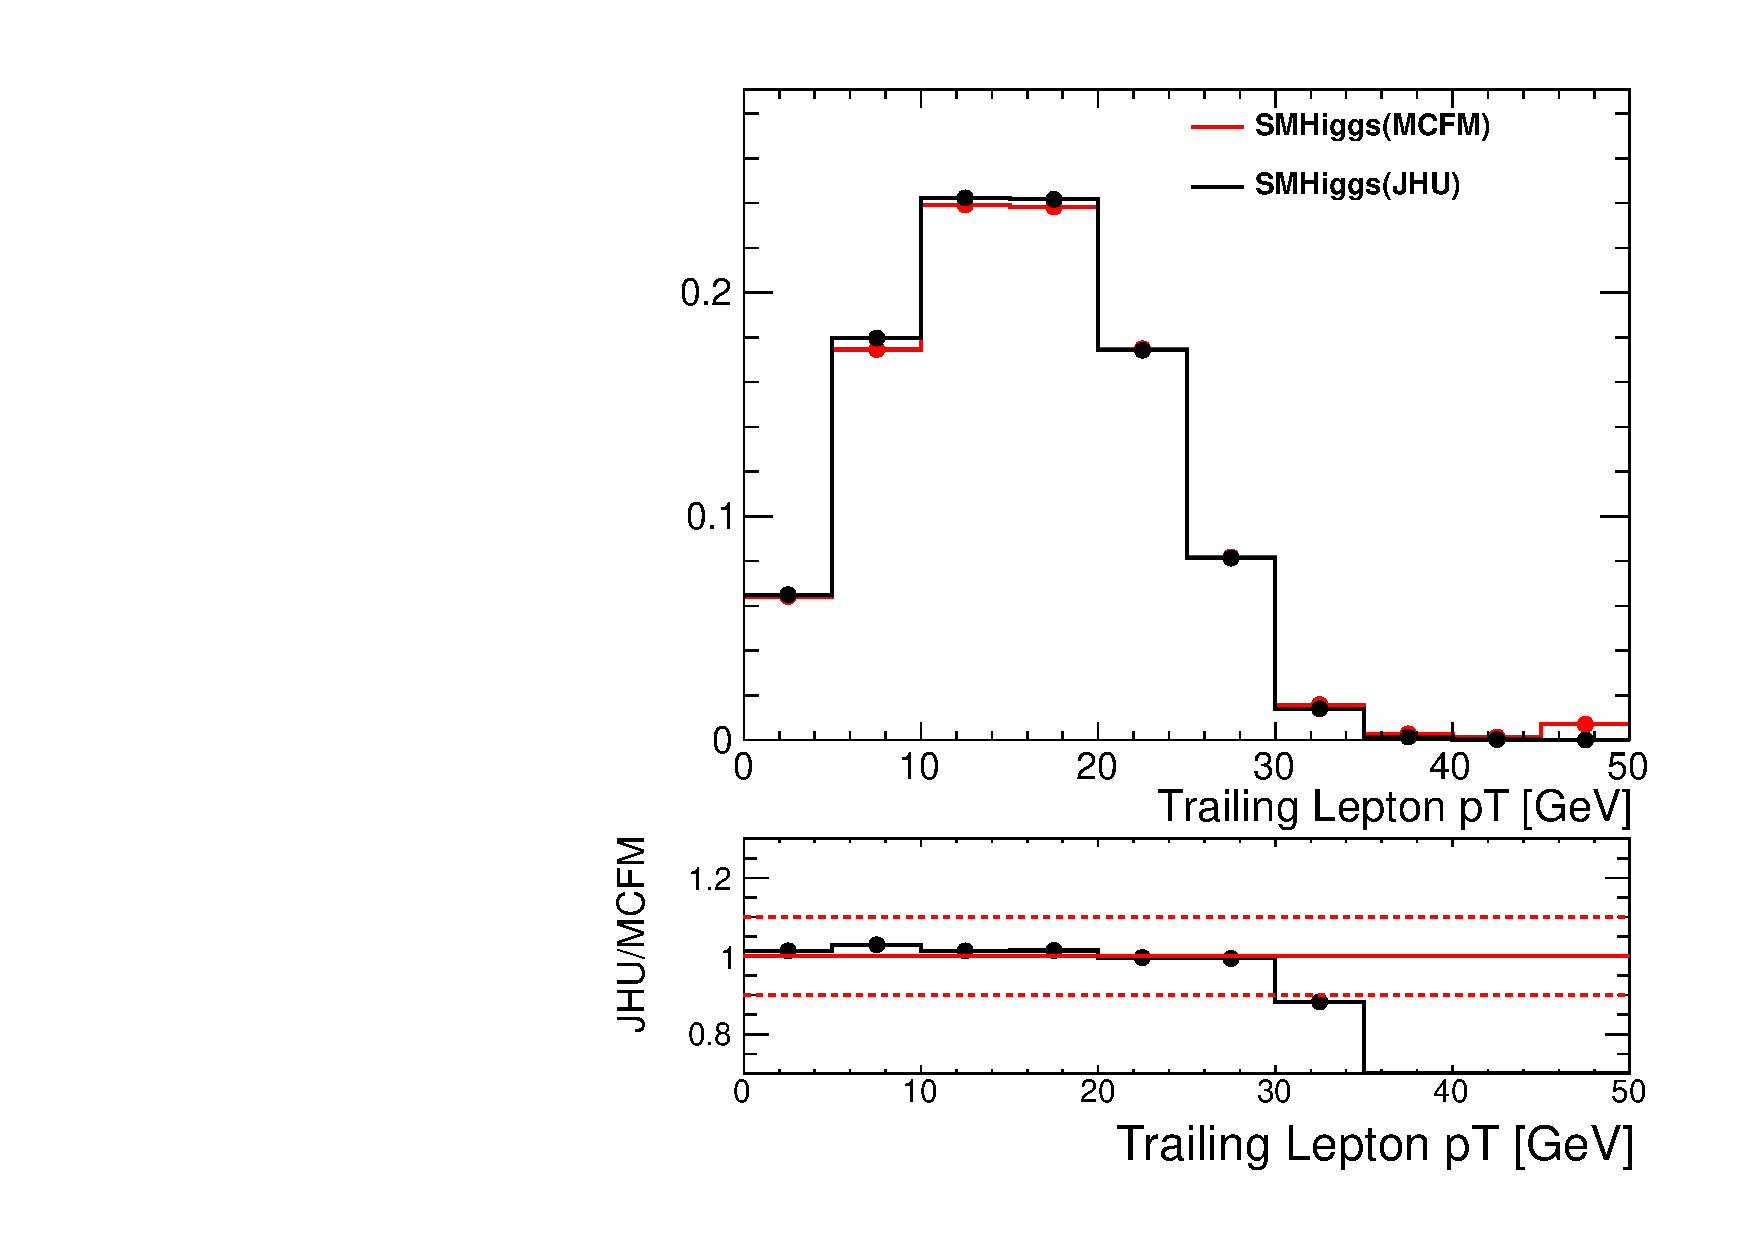
\includegraphics[width=.3\textwidth]{figures/trailleppt_jhuvsmcfm.pdf}
}
\subfigure[Leading Lepton $\eta$]{
\centering
\label{subfig:leadlepeta}
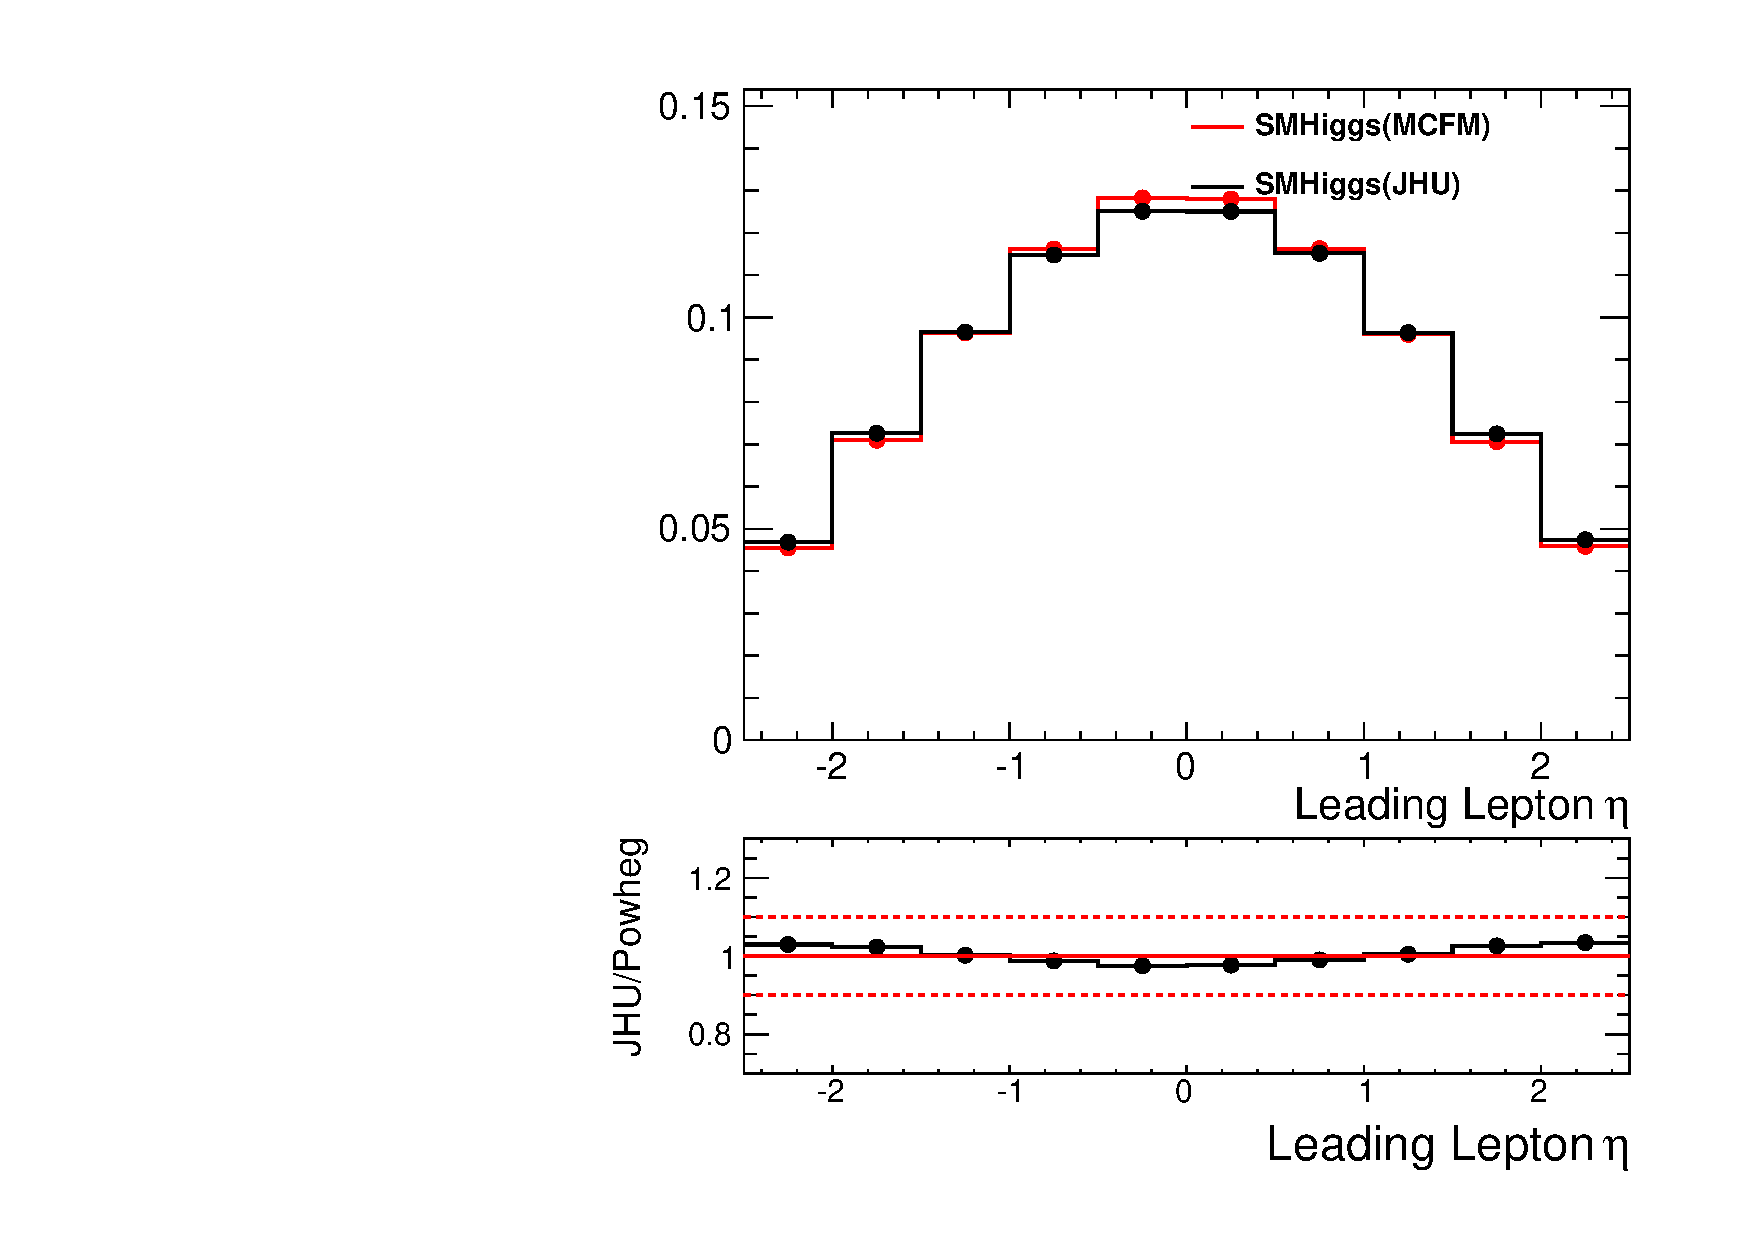
\includegraphics[width=.3\textwidth]{figures/leadlepeta_jhuvsmcfm.pdf}
} \\
\subfigure[Trailing Lepton $\eta$]{
\centering
\label{subfig:traillepeta}
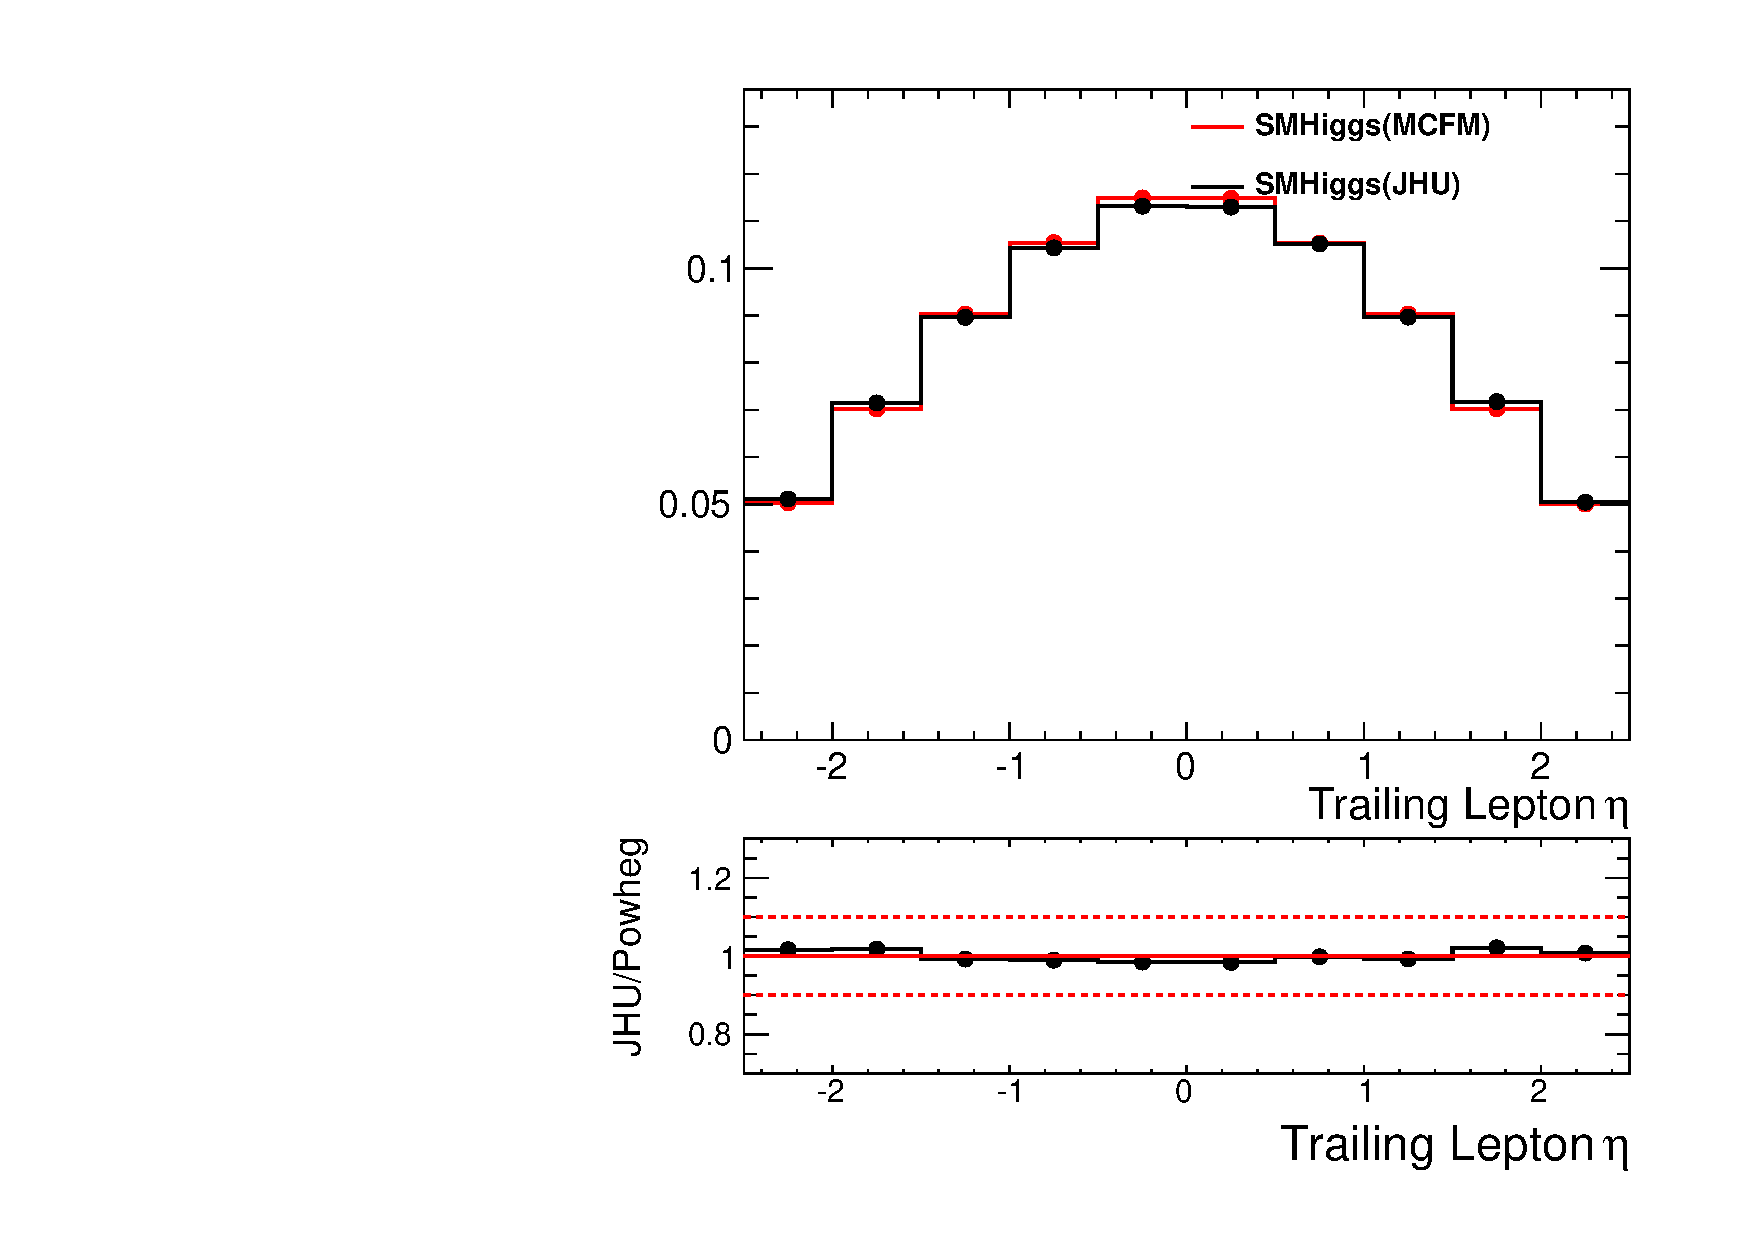
\includegraphics[width=.3\textwidth]{figures/traillepeta_jhuvsmcfm.pdf}
}
\subfigure[Dilepton mass]{
\centering
\label{subfig:mll}
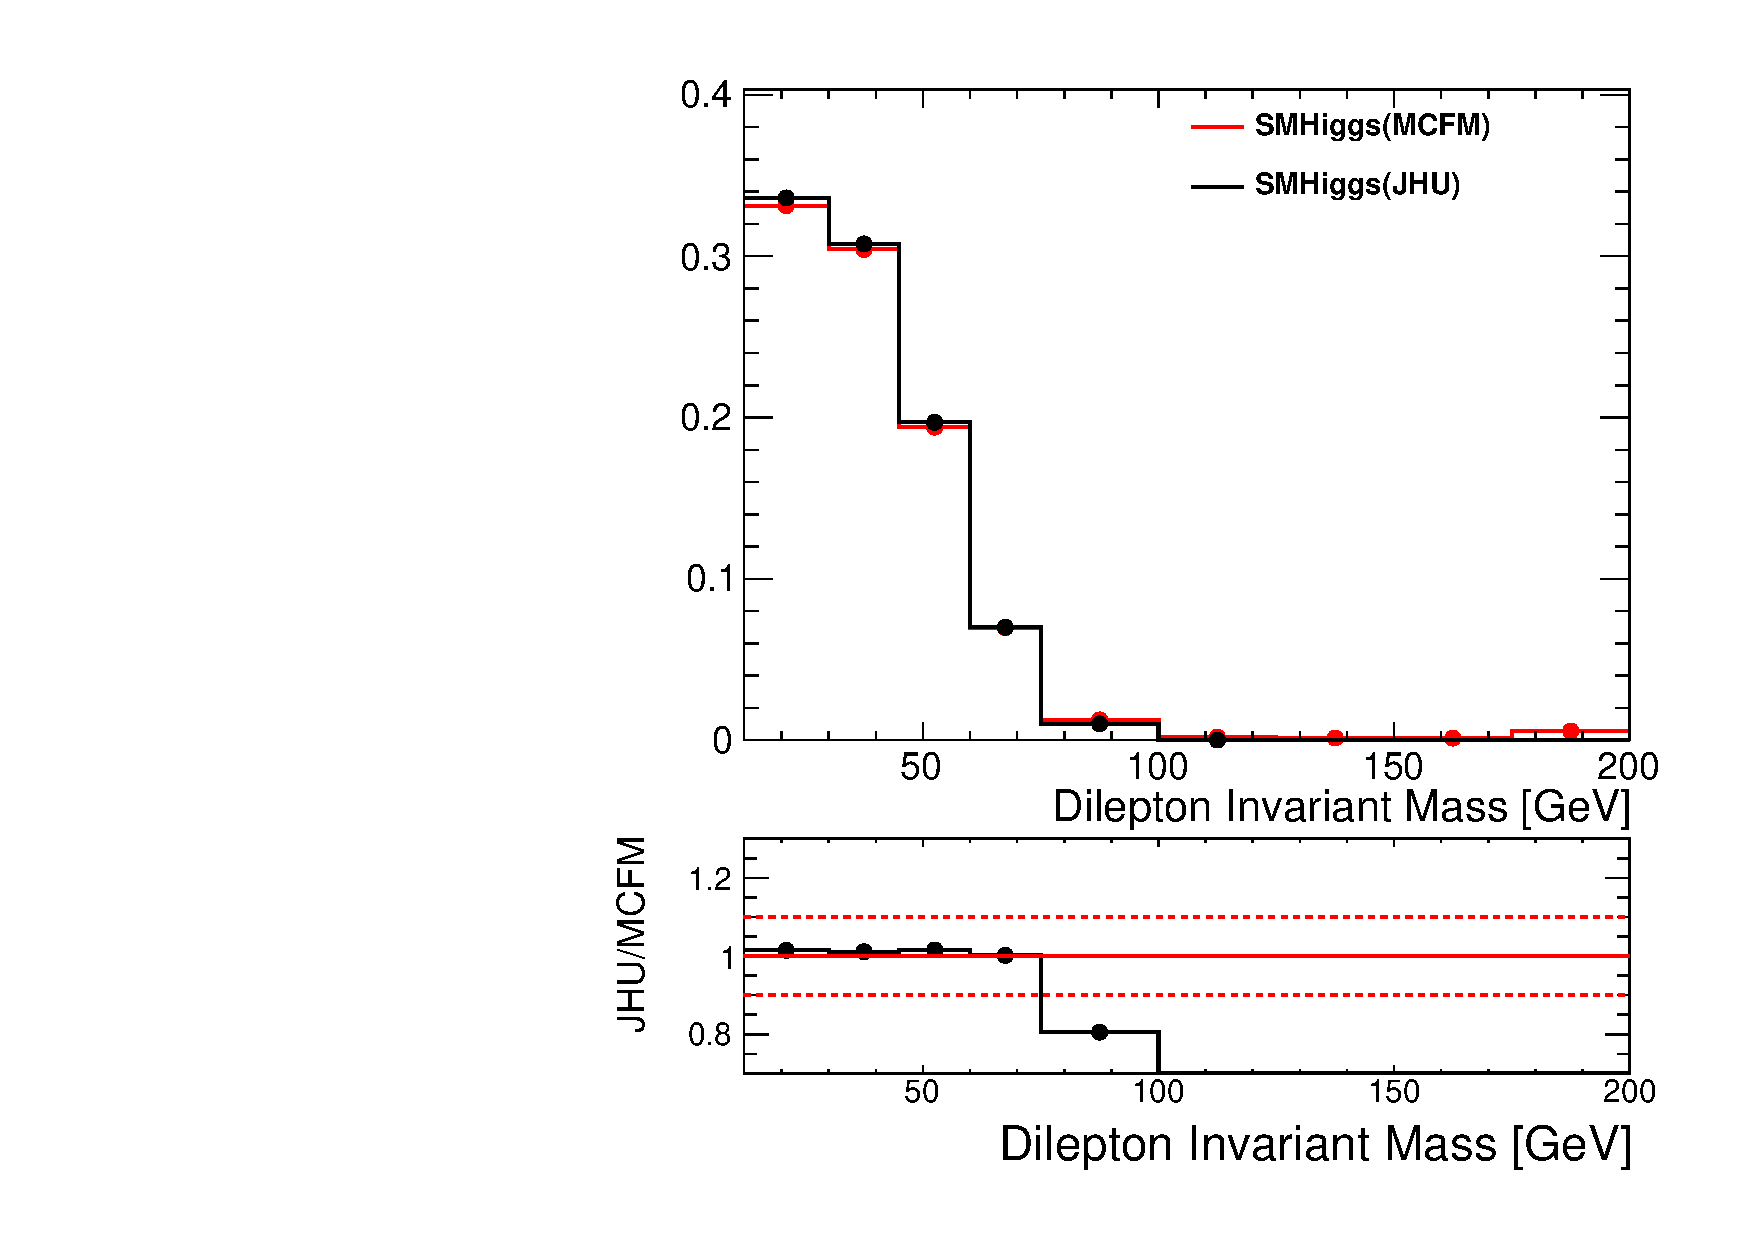
\includegraphics[width=.3\textwidth]{figures/mll_jhuvsmcfm.pdf}
} 
\subfigure[Transverse Higgs Mass]{
\centering
\label{subfig:mt}
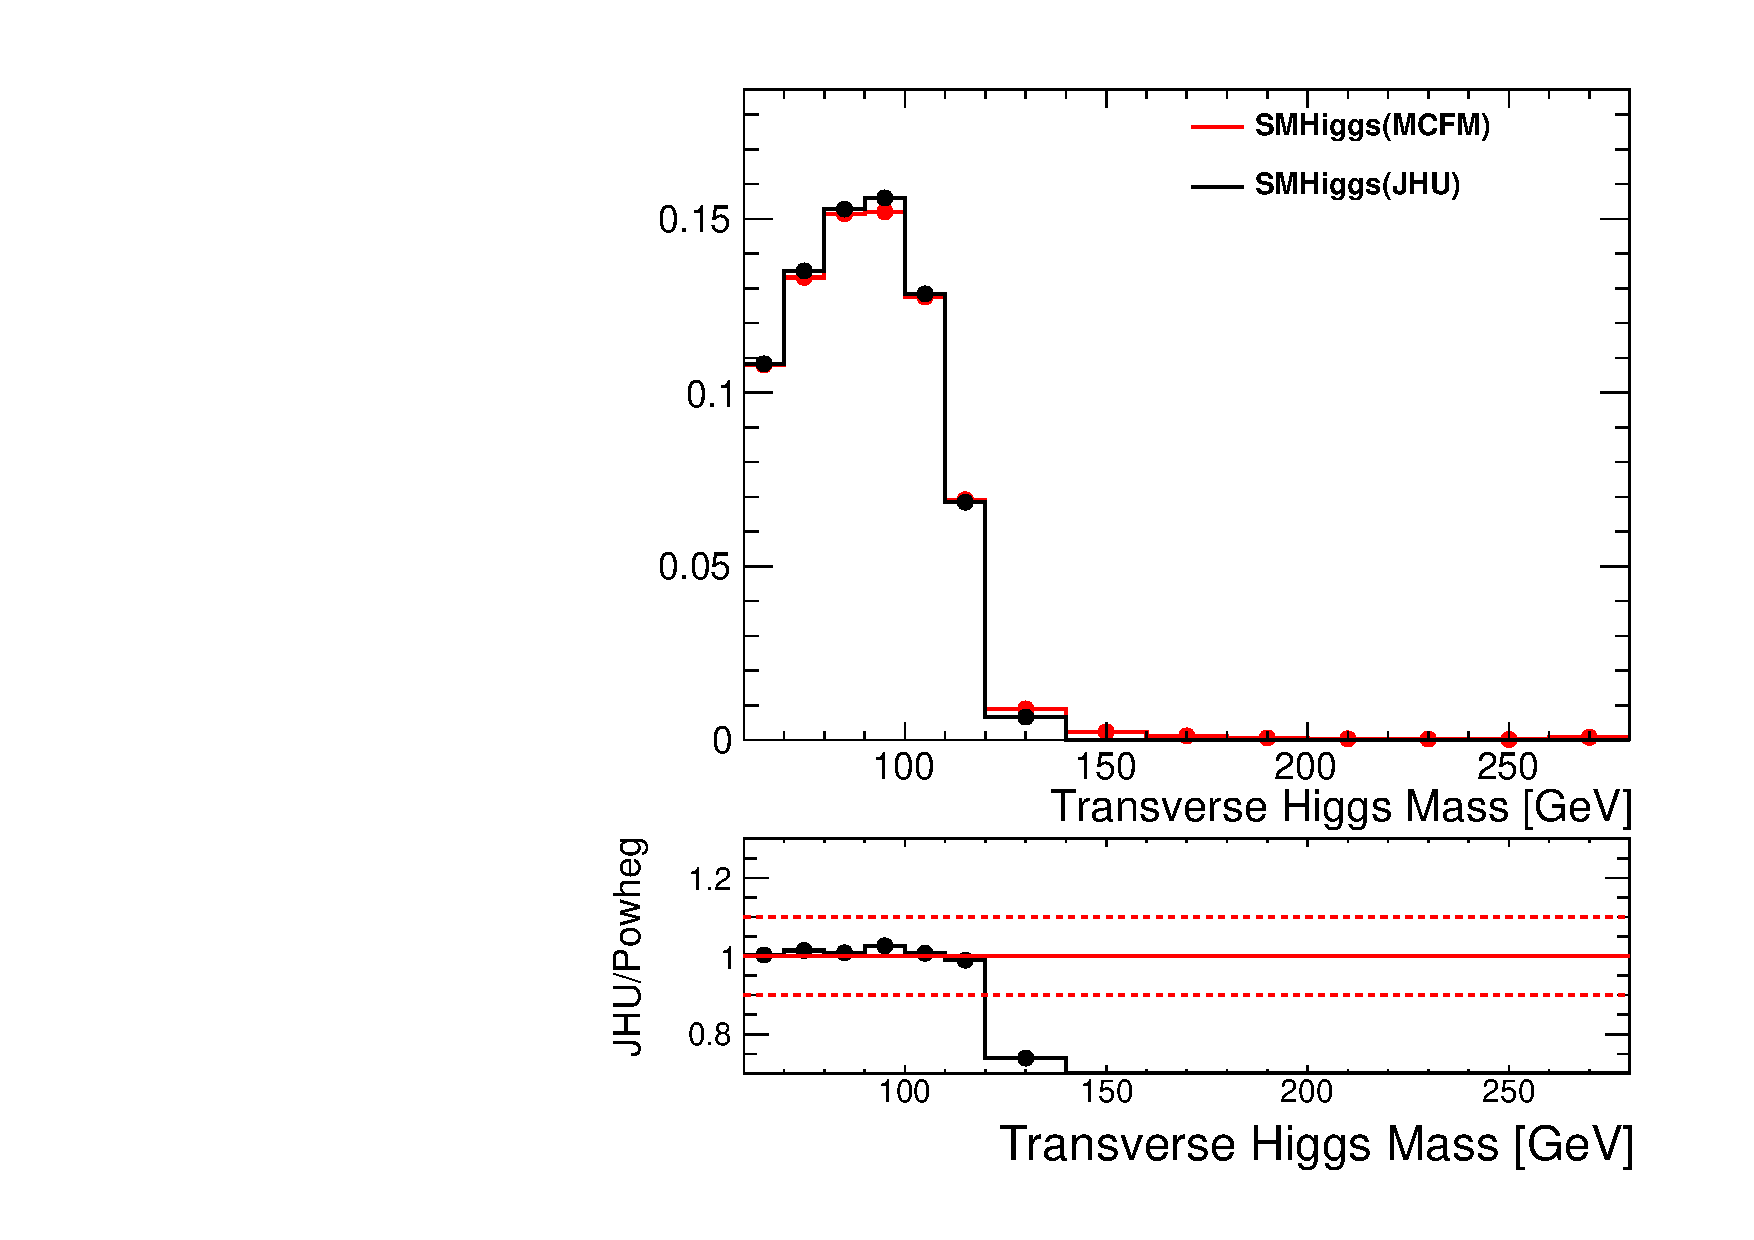
\includegraphics[width=.3\textwidth]{figures/mt_jhuvsmcfm.pdf}
}\\
\subfigure[Dilepton $\pt$]{
\centering
\label{subfig:dilpt}
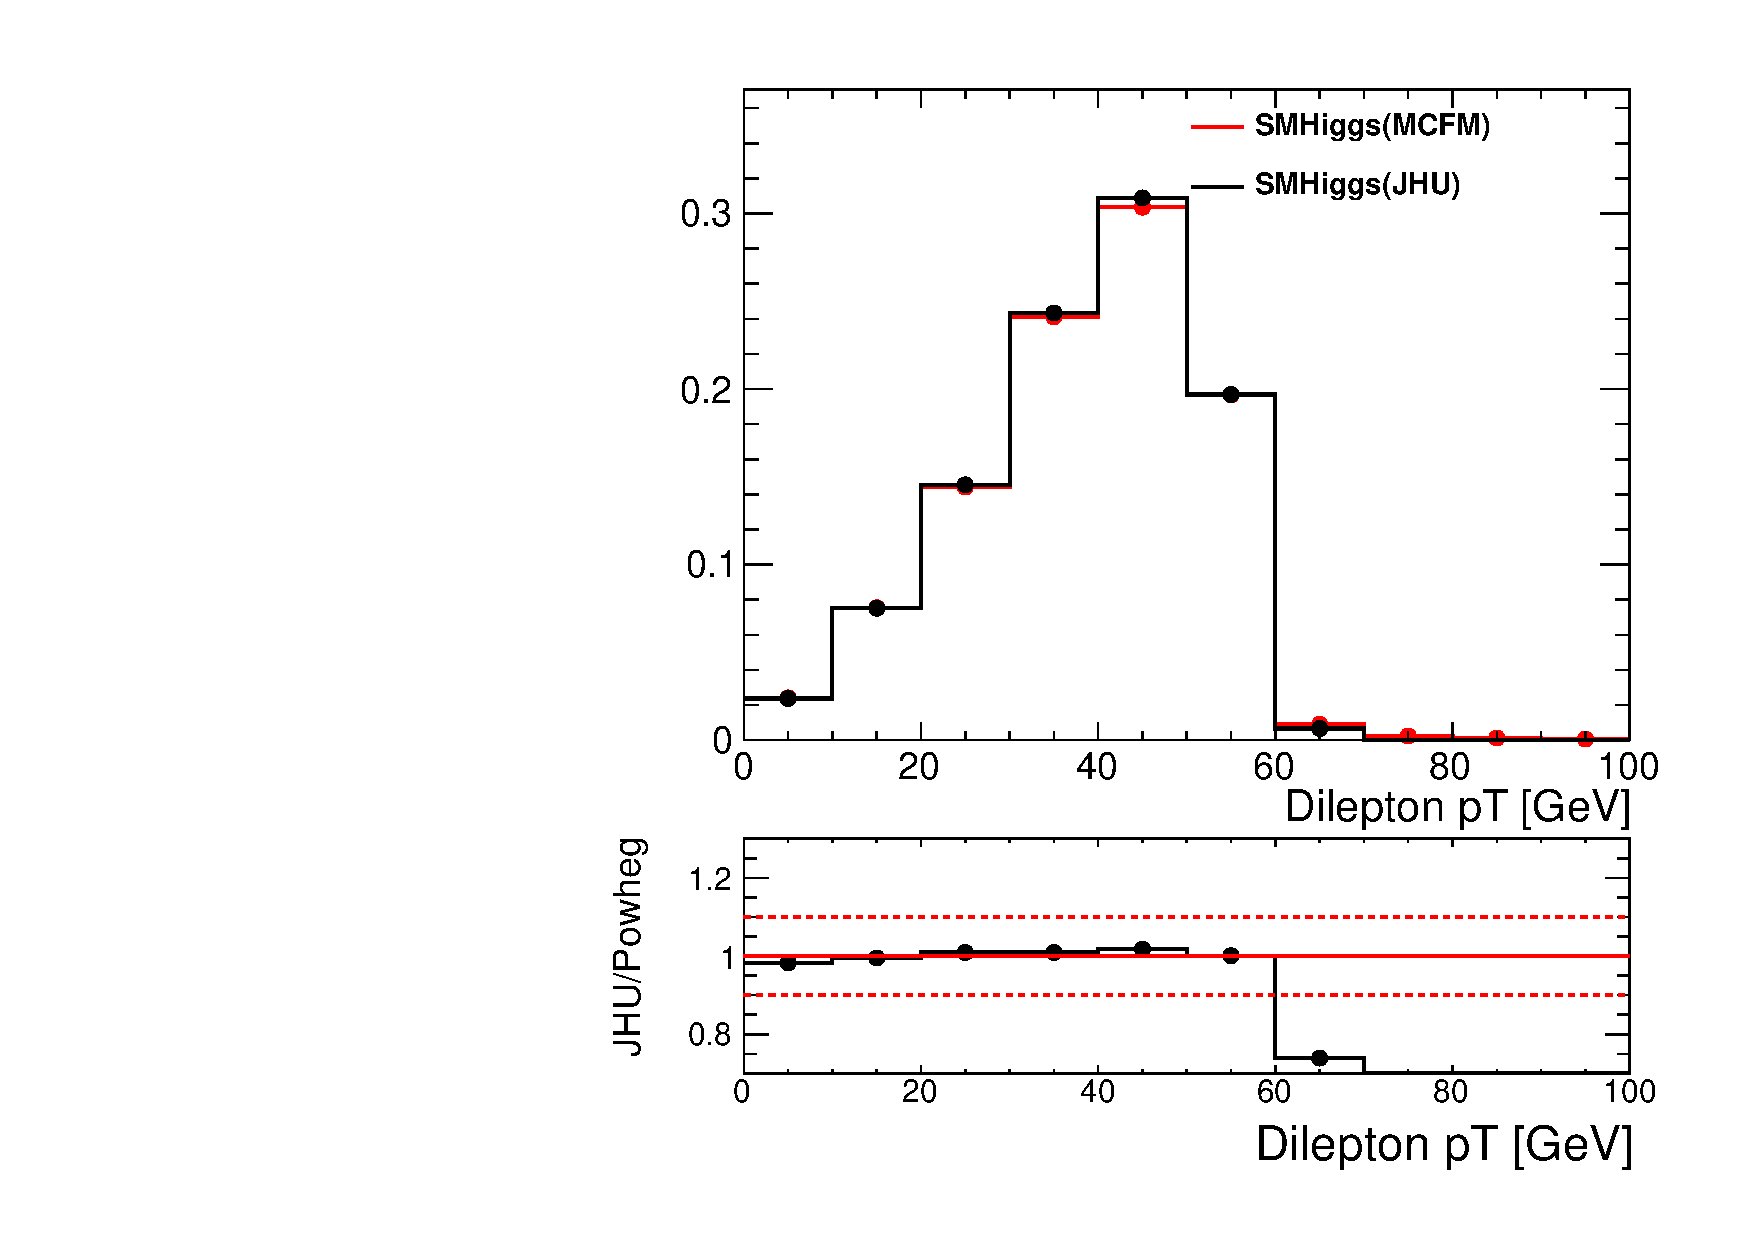
\includegraphics[width=.3\textwidth]{figures/dilpt_jhuvsmcfm.pdf}
}
\subfigure[Neutrino $\pt$]{
\centering
\label{subfig:met}
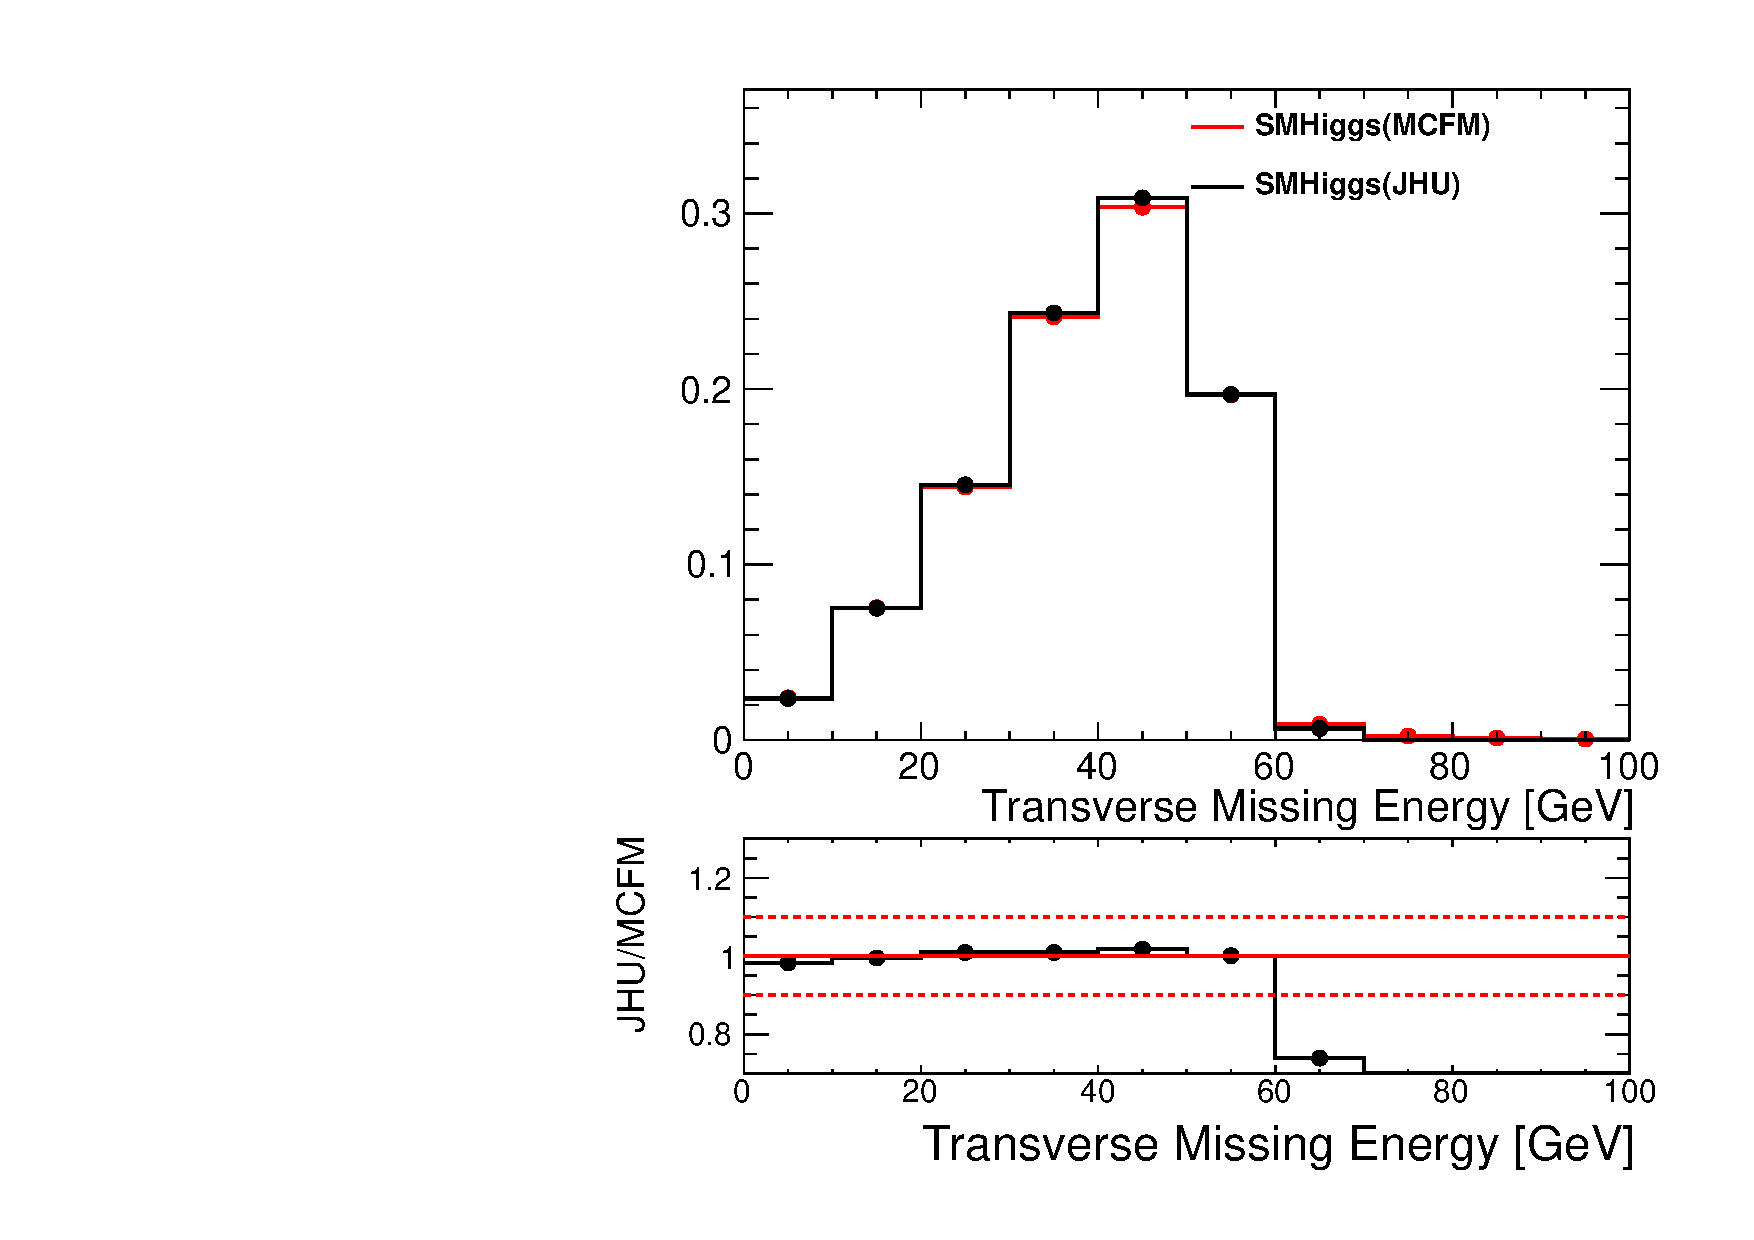
\includegraphics[width=.3\textwidth]{figures/met_jhuvsmcfm.pdf}
}
\subfigure[$\Delta\phi_{\ell\ell}$]{
\centering
\label{subfig:met}
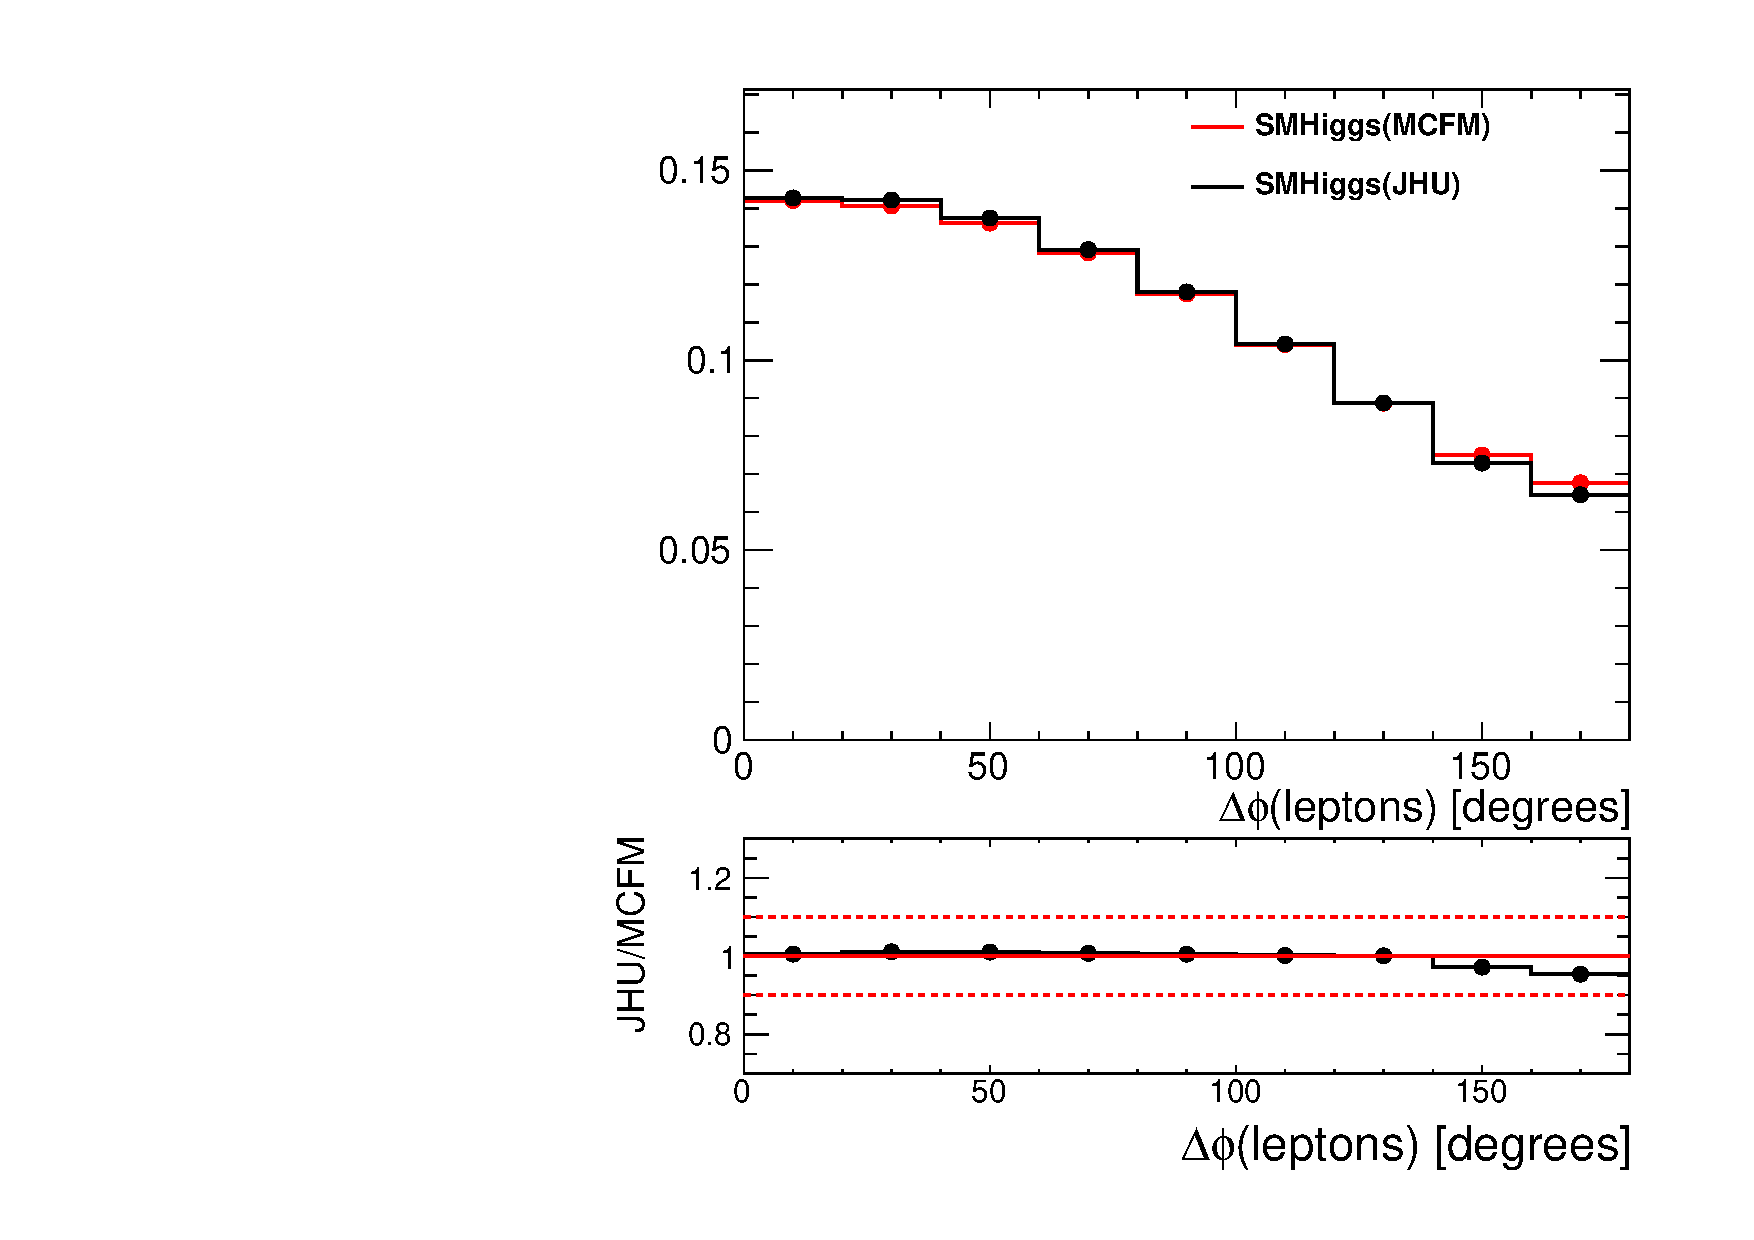
\includegraphics[width=.3\textwidth]{figures/dphill_jhuvsmcfm.pdf}
}\\
\caption{Gerator level kinematic distributions (normalized to 1) of SM Higgs 
comparing JHUGen and MCFM without any cuts. Both samples are generated with 
the Higgs boson produced at rest. }
\label{fig:jhuvsmcfm}
\end{figure}
%%%%%%%%%%%%%%%%%%%%%%%%%%%%%%%%%%%%%%%%%%%%%

Figure~\ref{fig:higgspt_0j} shows the Higgs boson $\pt$ and the leading jet 
$\pt$ distributions for the SM Higgs hypothesis comparing the 
JHUGen-Pythia and Powheg-Pythia~\cite{powheg} samples, after applying the full 
simulation, reconstruction and event selection. The two generators agree within 10\%. 
This level of agreement is expected because Powheg uses
NLO matrix element calculations. The effect on the main kinematic observables due to 
the difference in Higgs $\pt$ however is smaller, as shown in Figure~\ref{fig:higgskin_0j}. 

%To account for the missing higher order effects in JHUGen,
%we reweight the two-dimensional templates ($m_T-m_{\ell\ell}$) 
%in the final analysis from JHUGen-Pythia to match to the predictions of Powheg-Pythia for the SM Higgs hypothesis. 
%The relative difference between JHUGen and Powheg in the SM Higgs boson hypothesis is then applied to the other signal hypotheses as well, because we 
%assume the effects are similar as all resonances are colorless objects. 
%%Therefore the missing higher 
%order effects are similar between different hypotheses. 
Figure~\ref{fig:gravvshiggspt_0j} shows the resonance $\pt$ and 
the leading jet $\pt$ distributions comparing the spin-2 
graviton and the SM Higgs hypothesis generated with the JHUGen-Pythia. 
The two hypotheses agree within a few percent in the bulk of the distributions,
smaller than the differences between Powheg-Pythia and JHUGen-Pythia 
in the SM Higgs hypothesis. 
For the moment we use the same theoretical uncertainties as in the SM Higgs 
analysis for the $2_{\text min}^+$ analysis..
%An additional systematic uncertainty due to this difference is assigned,
%as described in Section~\ref{sec:systematics}. 

%%%%%%%%%%%%%%%%%%%%%%%%%%%%%%%%%%%%%%%%%%%%%
\begin{figure}[!hbtp]
\centering
\subfigure[Higgs $\pt$]{
\centering
\label{subfig:higgspt_0j}
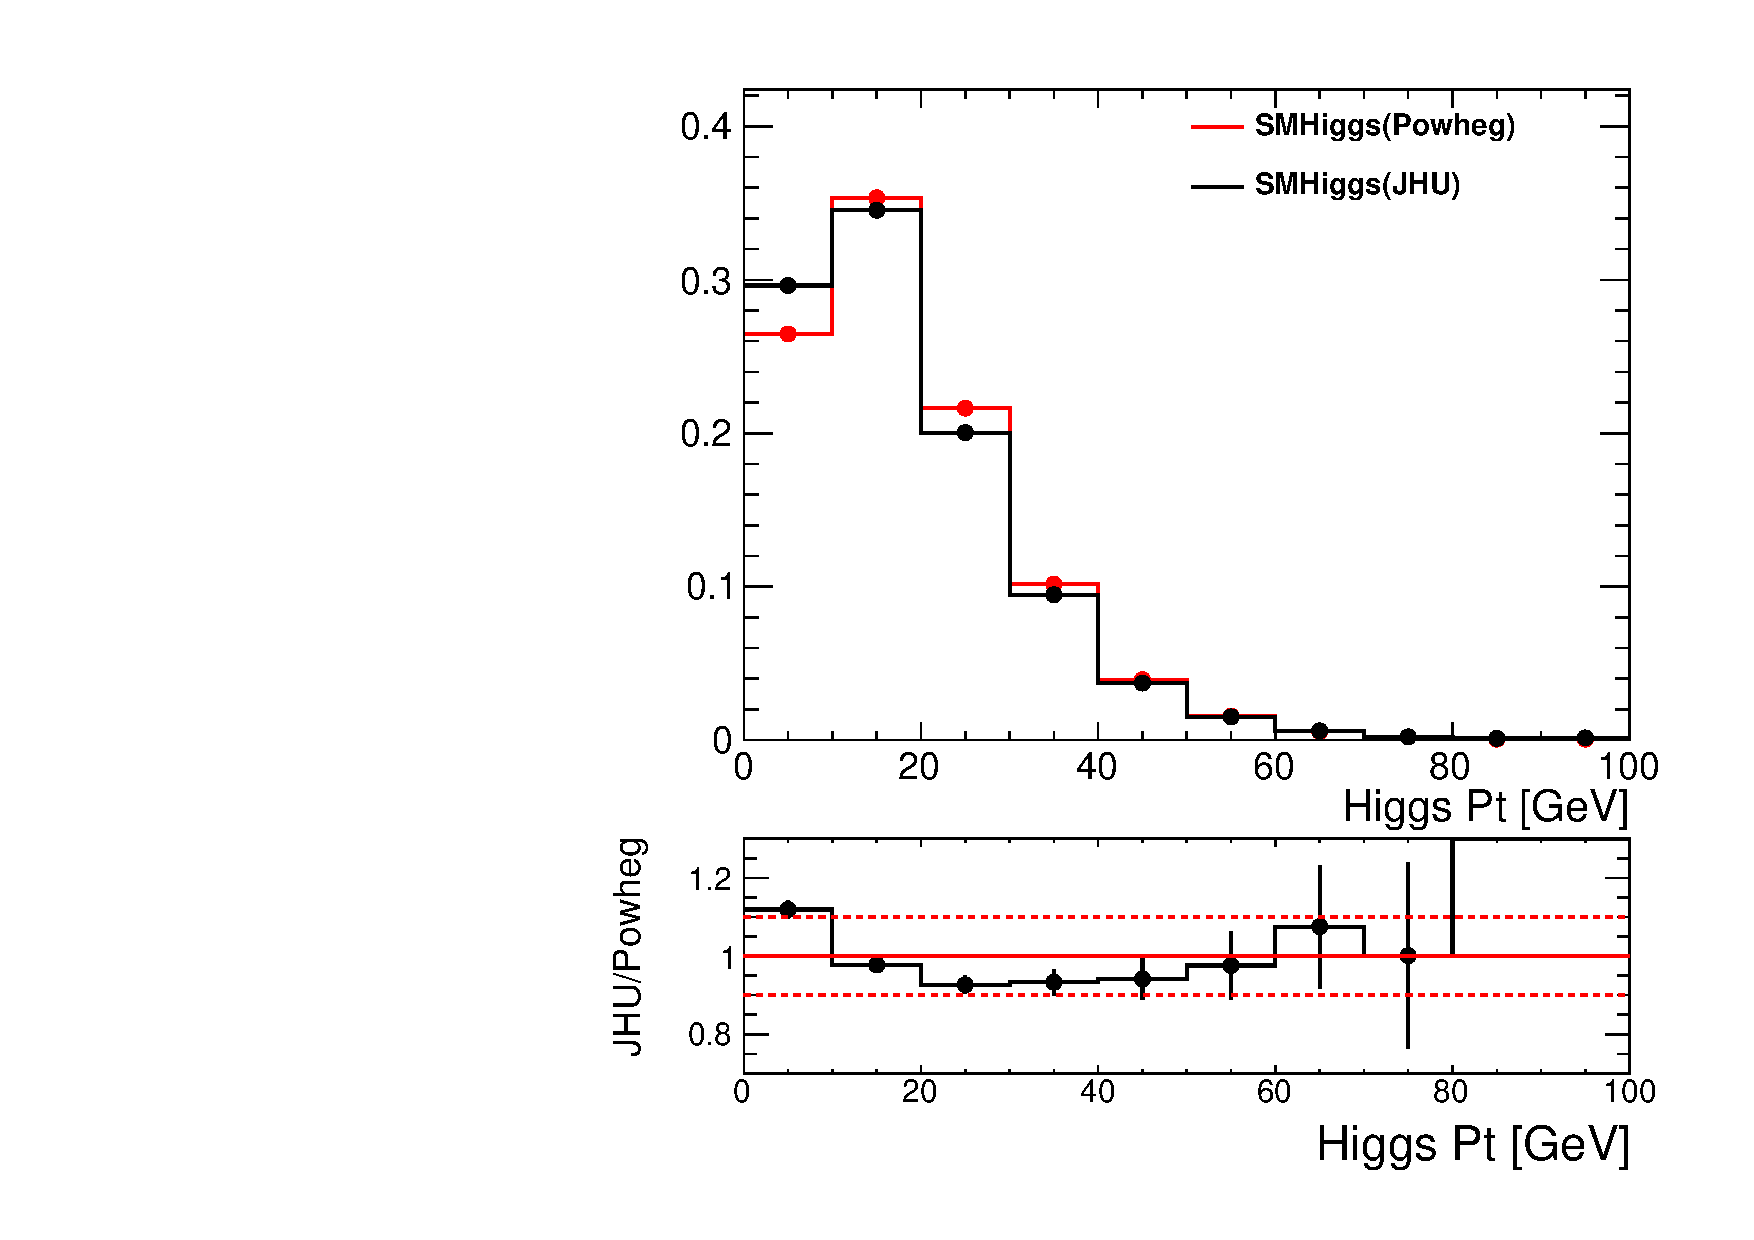
\includegraphics[width=.3\textwidth]{figures/higgsPt.pdf}
}
\subfigure[Leading Jet $\pt$]{
\centering
\label{subfig:jet1pt_0j}
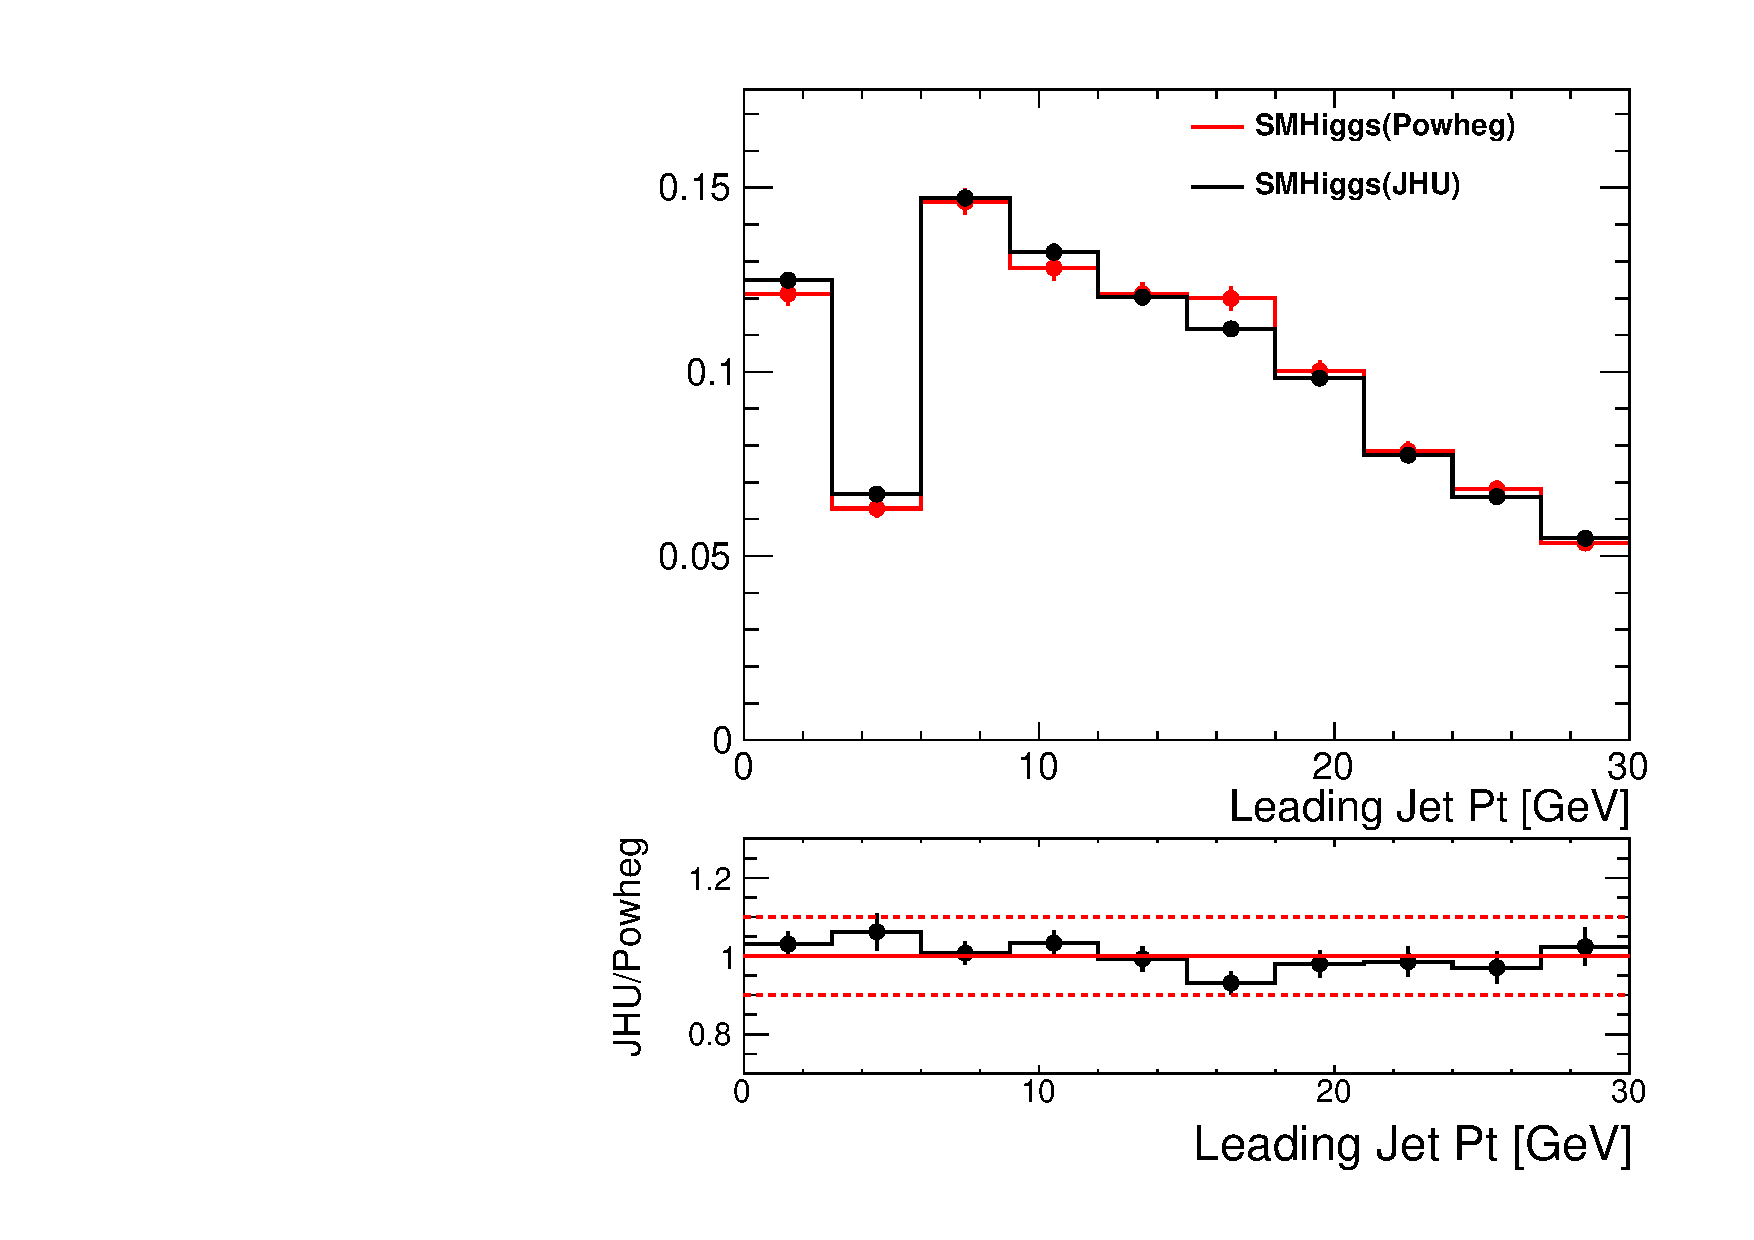
\includegraphics[width=.3\textwidth]{figures/jet1pt.pdf}
}\\
\caption{The Higgs $\pt$ and the leading jet $\pt$ distributions (normalized to 1) of the 
SM Higgs hypothesis comparing the powheg generator and JHUGen, after 
applying the final event selections. }
\label{fig:higgspt_0j}
\end{figure}
%%%%%%%%%%%%%%%%%%%%%%%%%%%%%%%%%%%%%%%%%%%%%


%%%%%%%%%%%%%%%%%%%%%%%%%%%%%%%%%%%%%%%%%%%%%
\begin{figure}[!hbtp]
\centering
\subfigure[Leading Lepton $\pt$]{
\centering
\label{subfig:leadleppt}
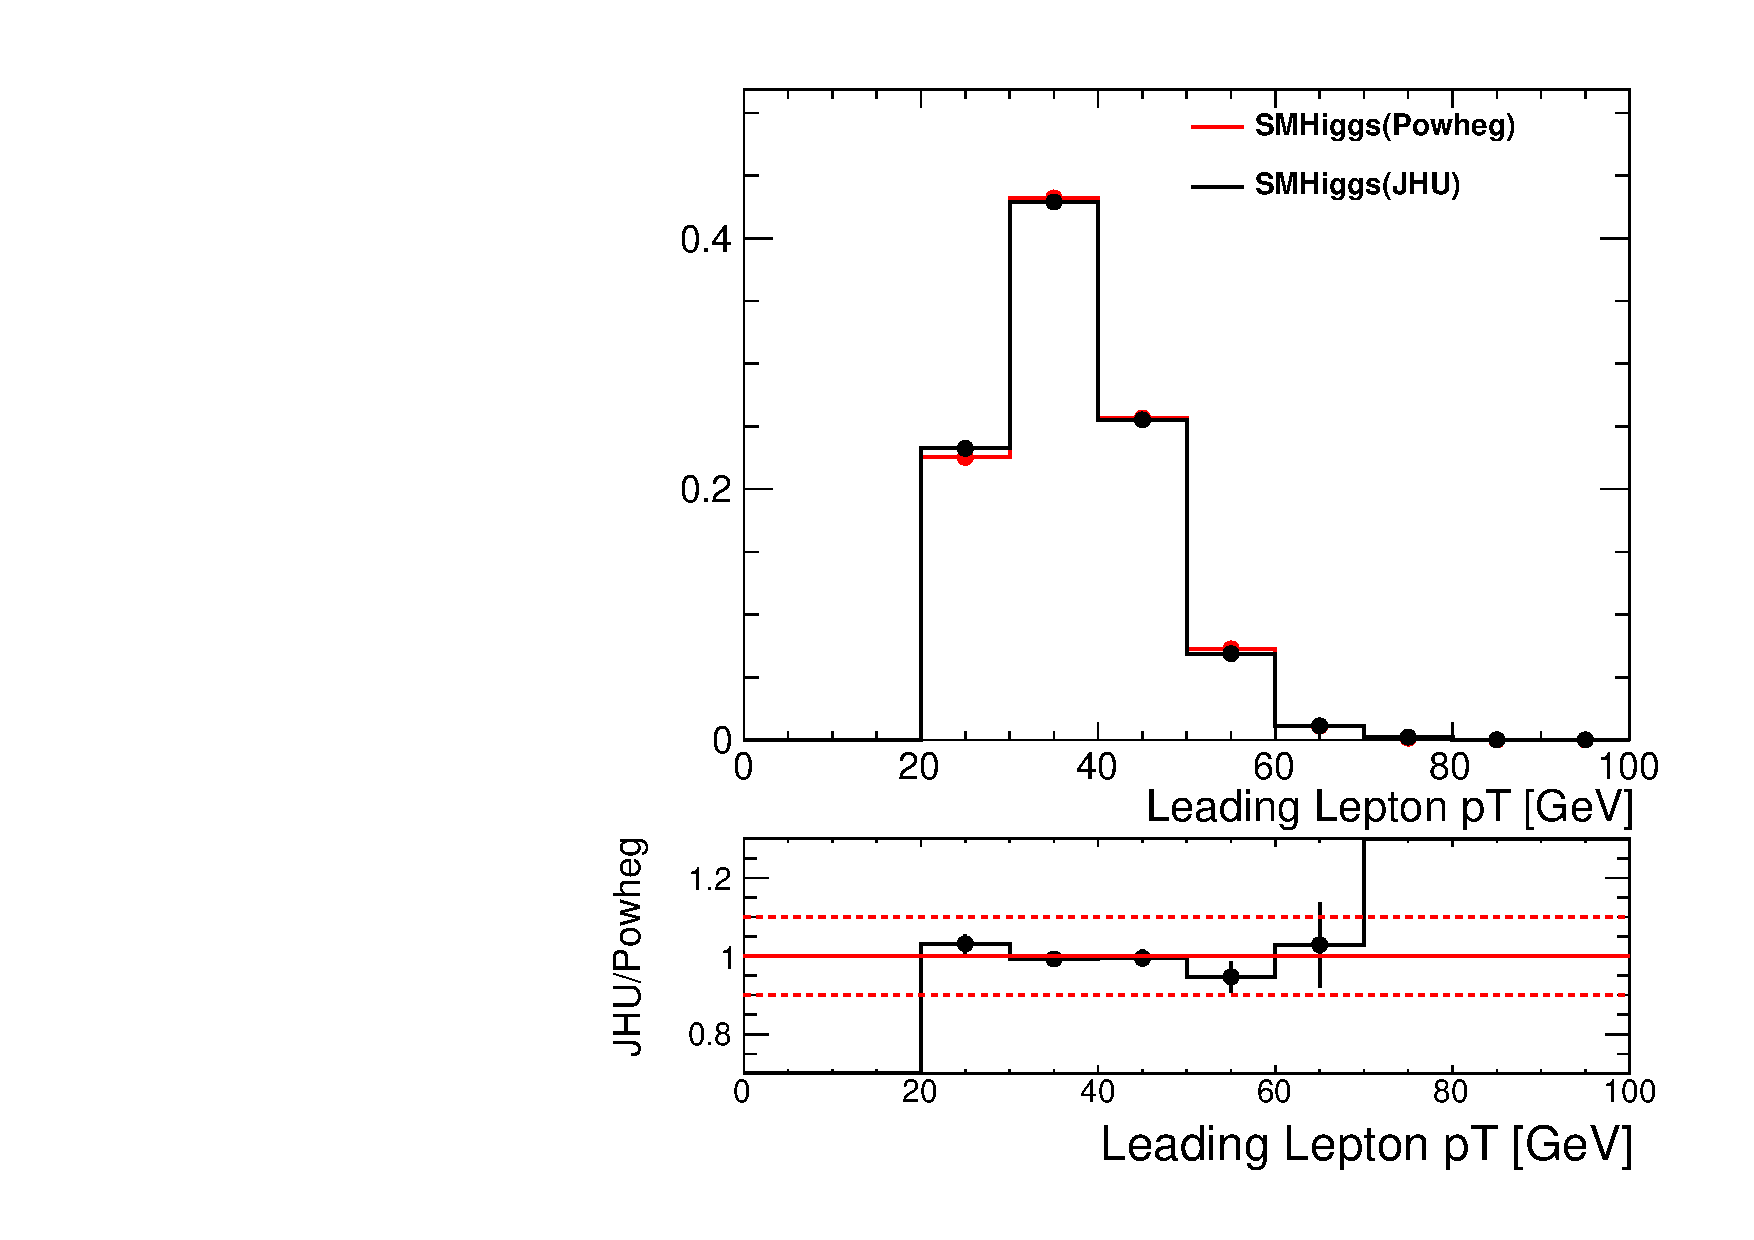
\includegraphics[width=.3\textwidth]{figures/leadleppt.pdf}
}
\subfigure[Trailing Lepton $\pt$]{
\centering
\label{subfig:trailleppt}
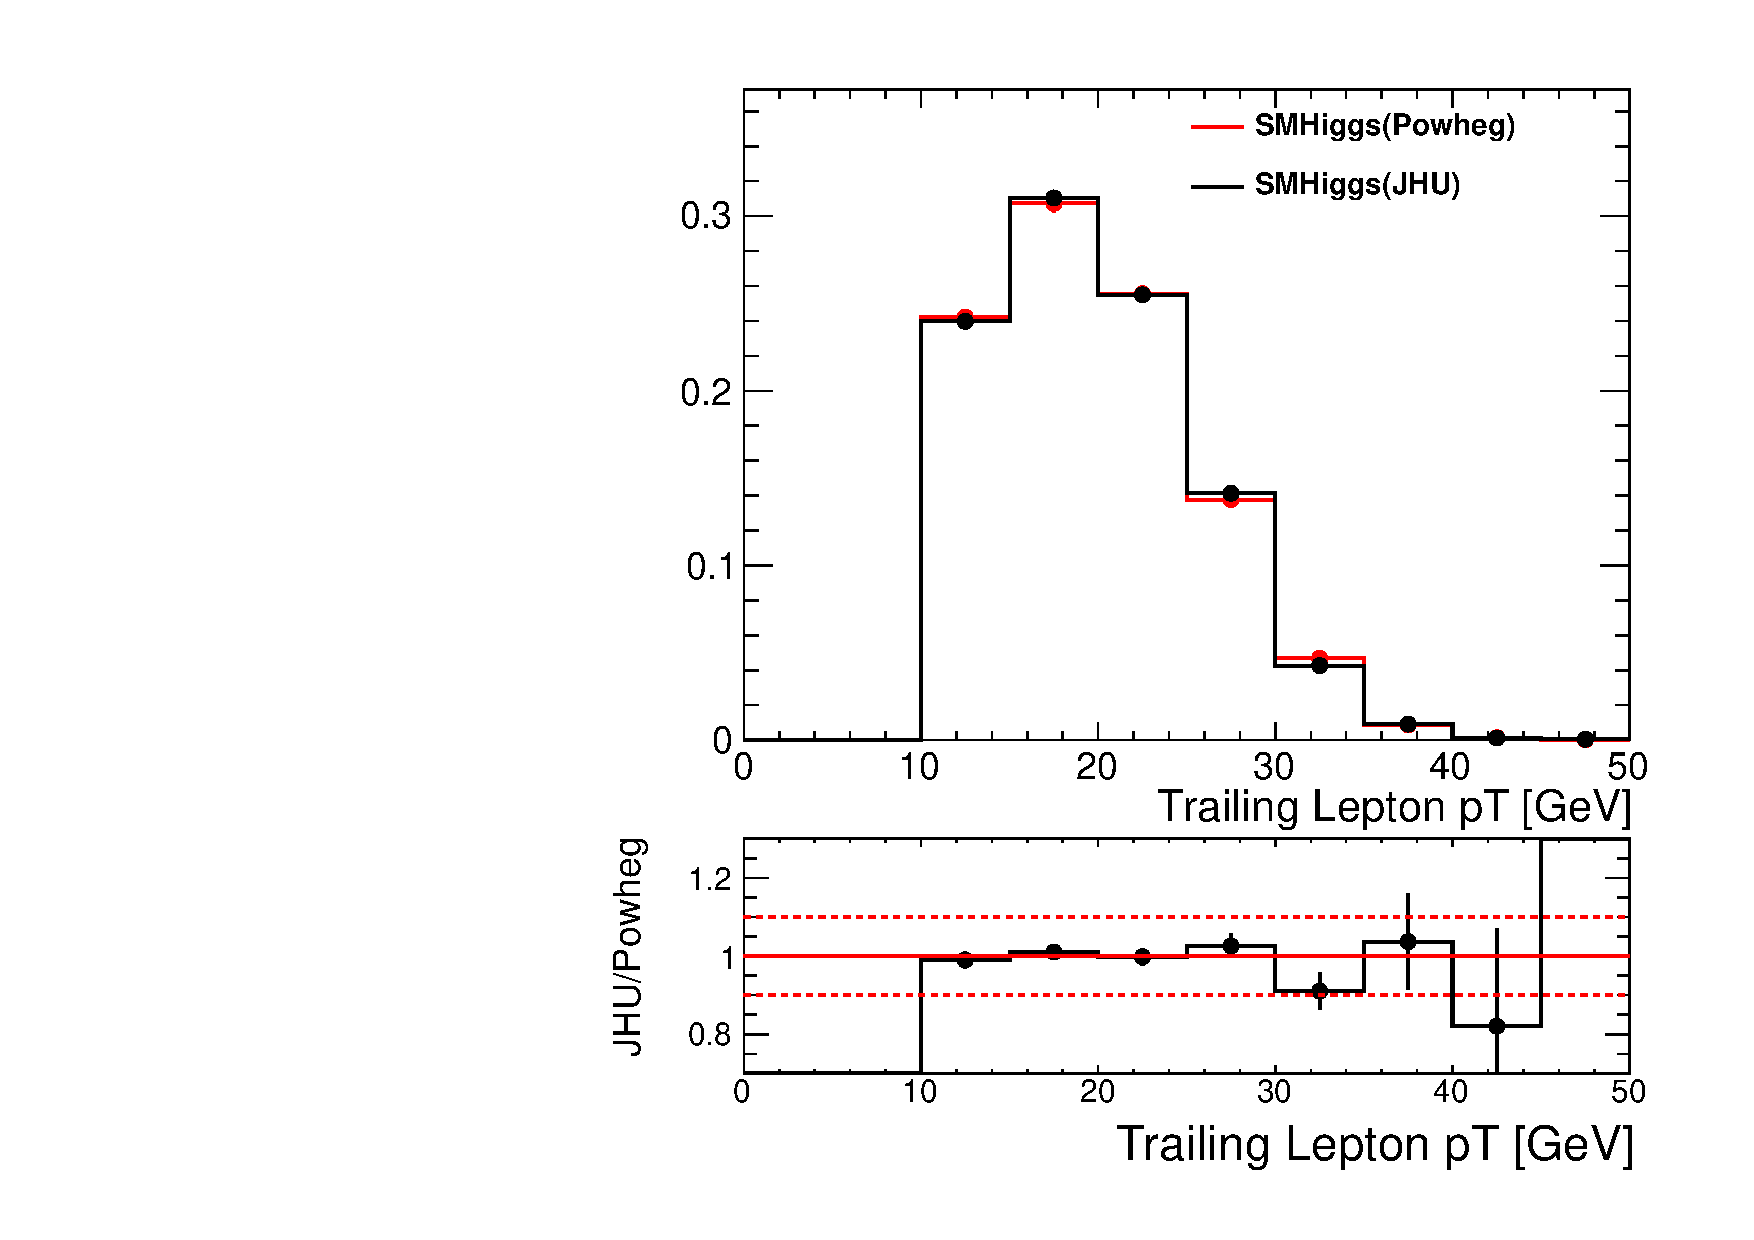
\includegraphics[width=.3\textwidth]{figures/trailleppt.pdf}
}
\subfigure[Leading Lepton $\eta$]{
\centering
\label{subfig:leadlepeta}
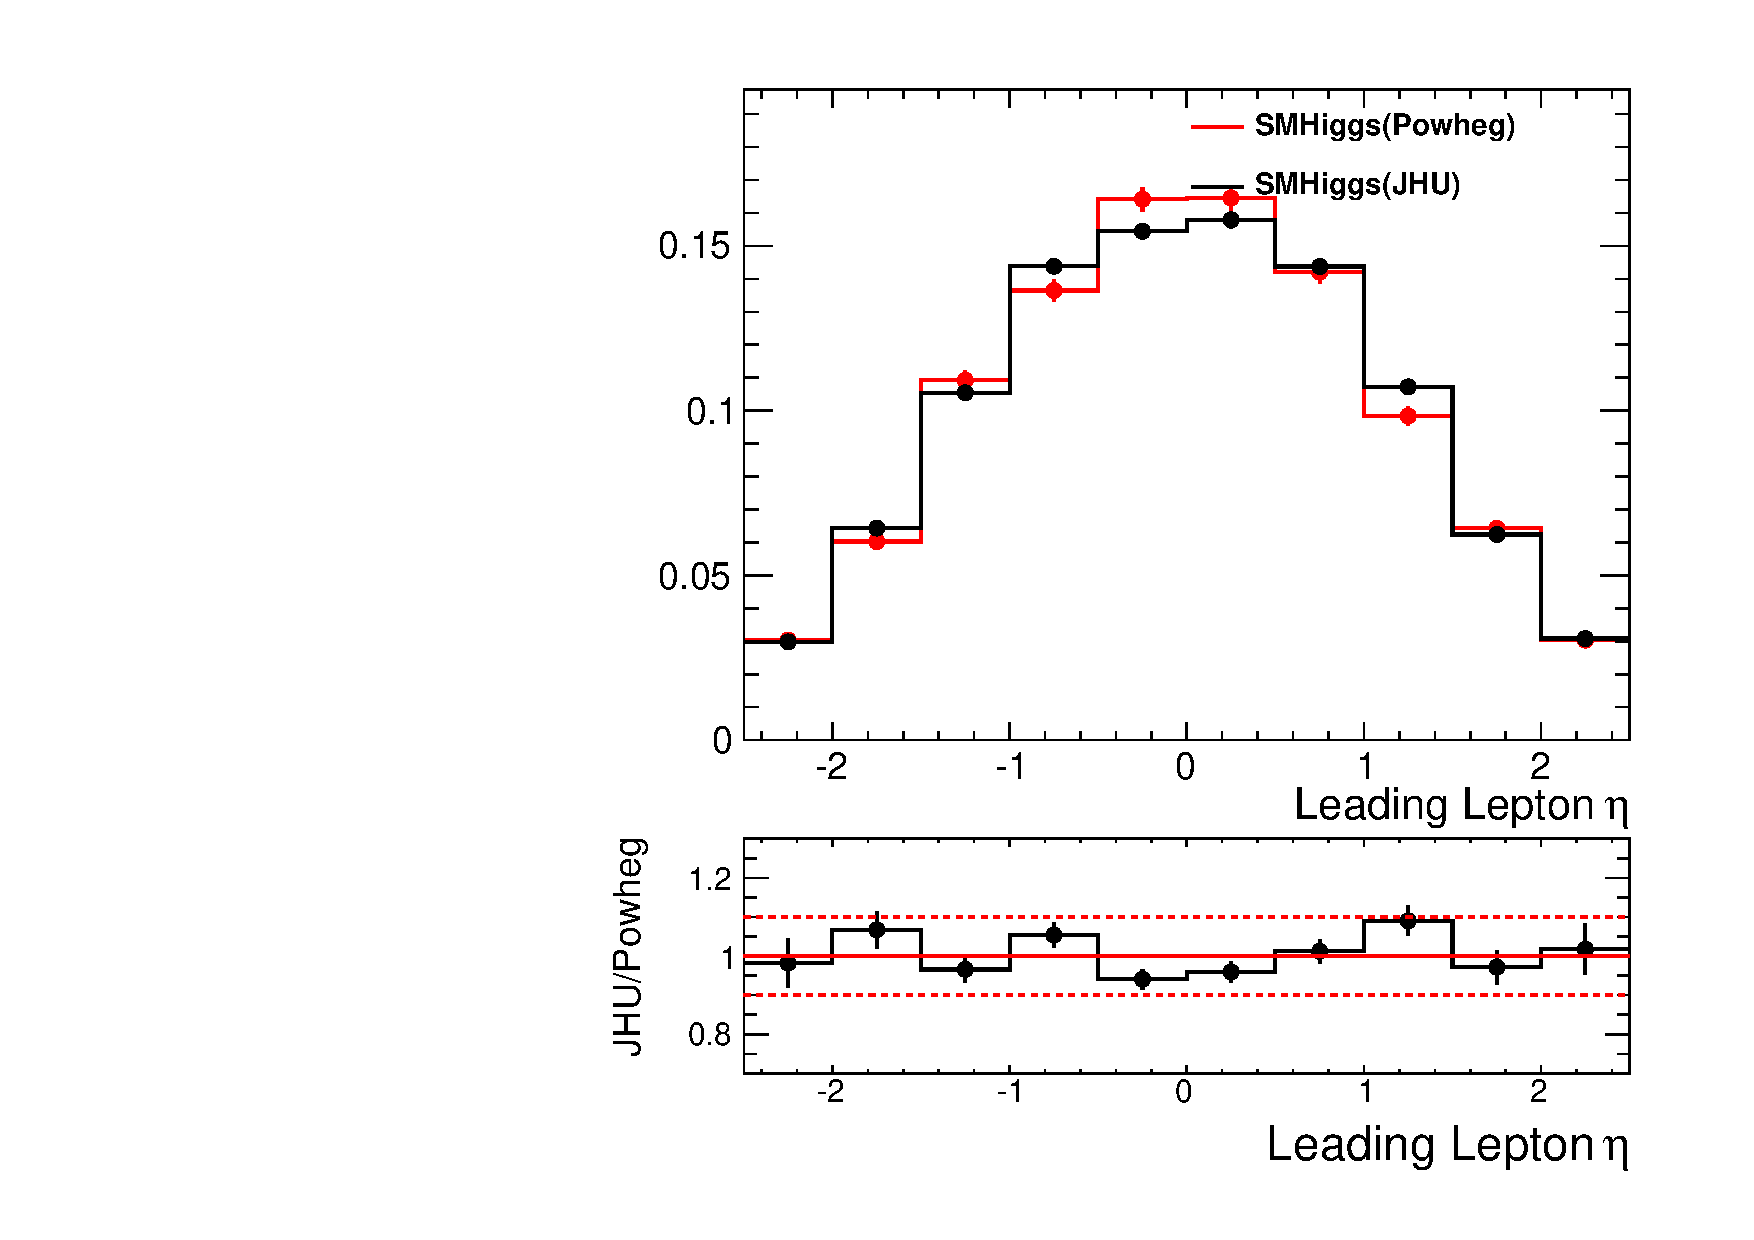
\includegraphics[width=.3\textwidth]{figures/leadlepeta.pdf}
} \\
\subfigure[Trailing Lepton $\eta$]{
\centering
\label{subfig:traillepeta}
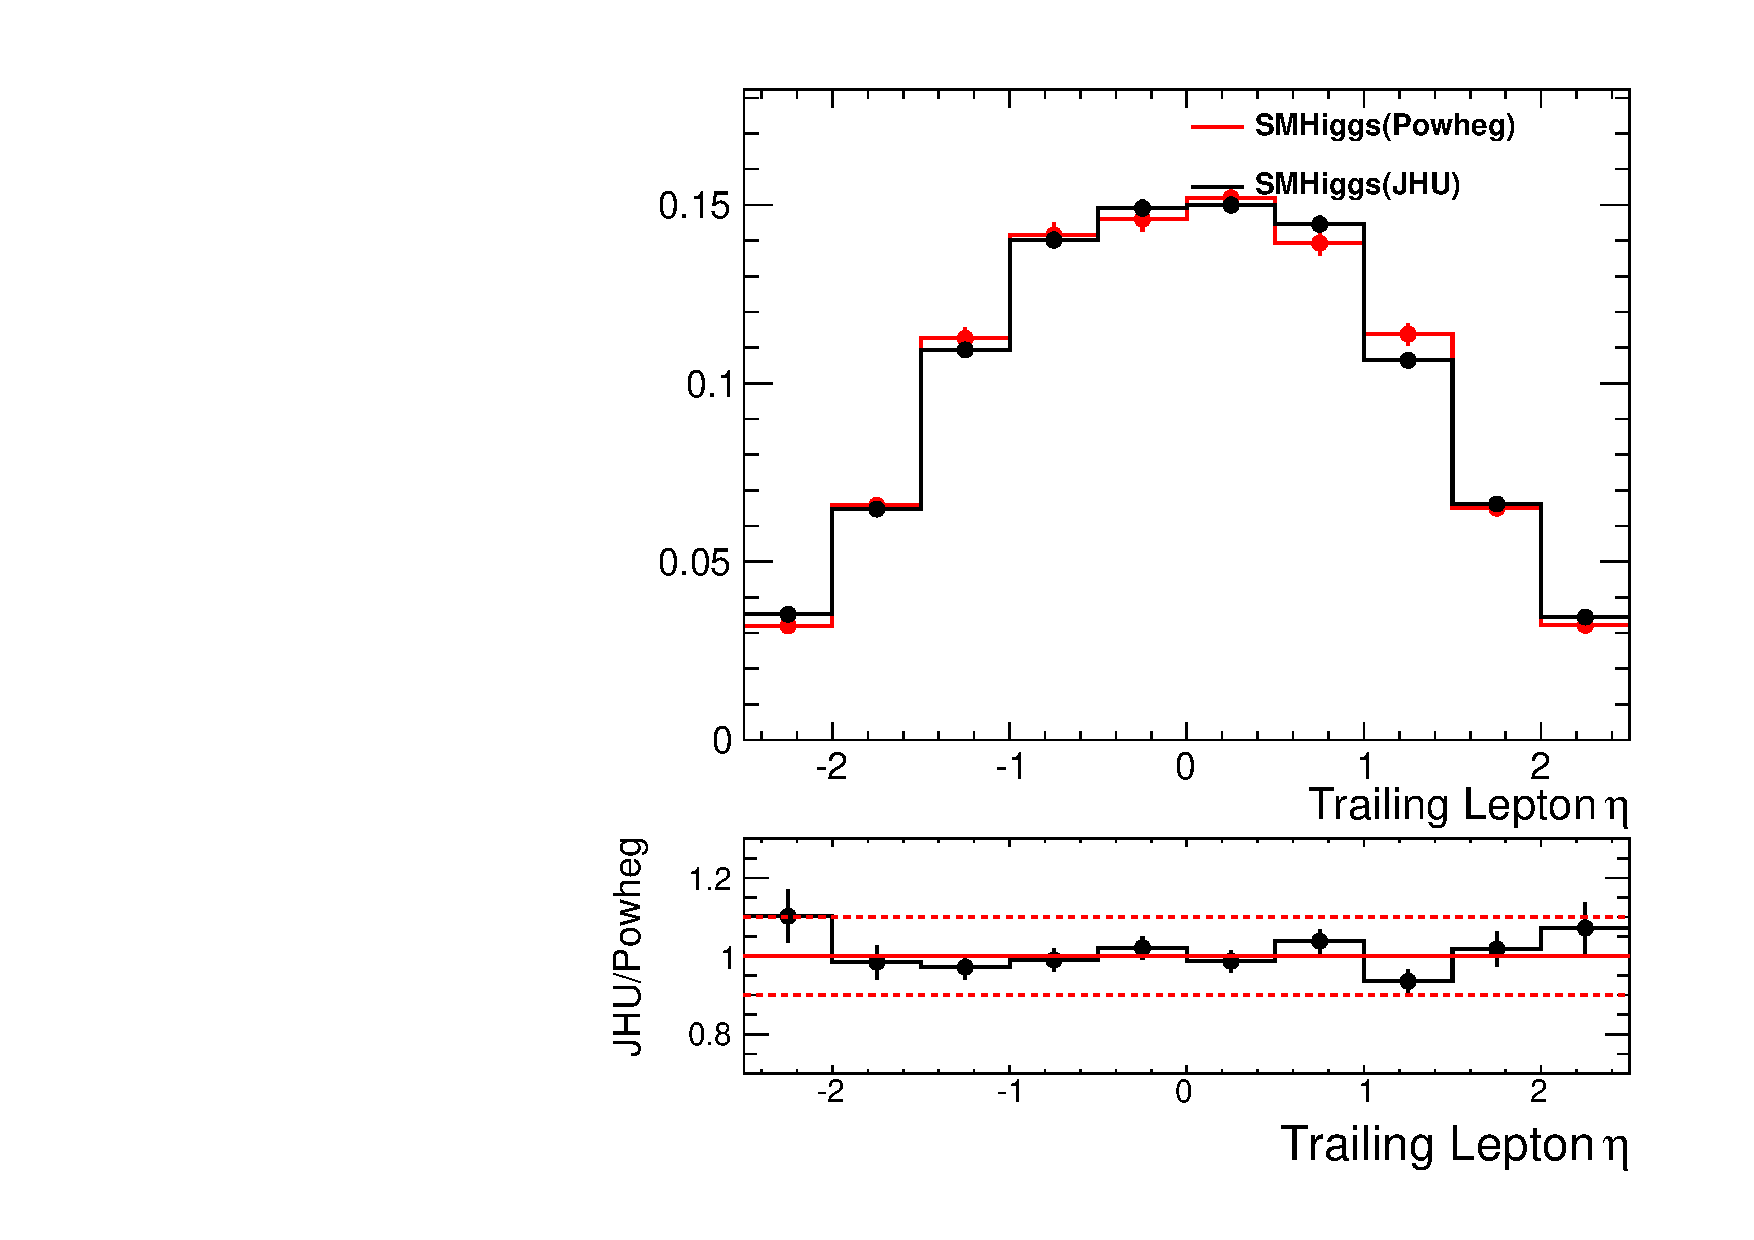
\includegraphics[width=.3\textwidth]{figures/traillepeta.pdf}
}
\subfigure[Dilepton mass]{
\centering
\label{subfig:mll}
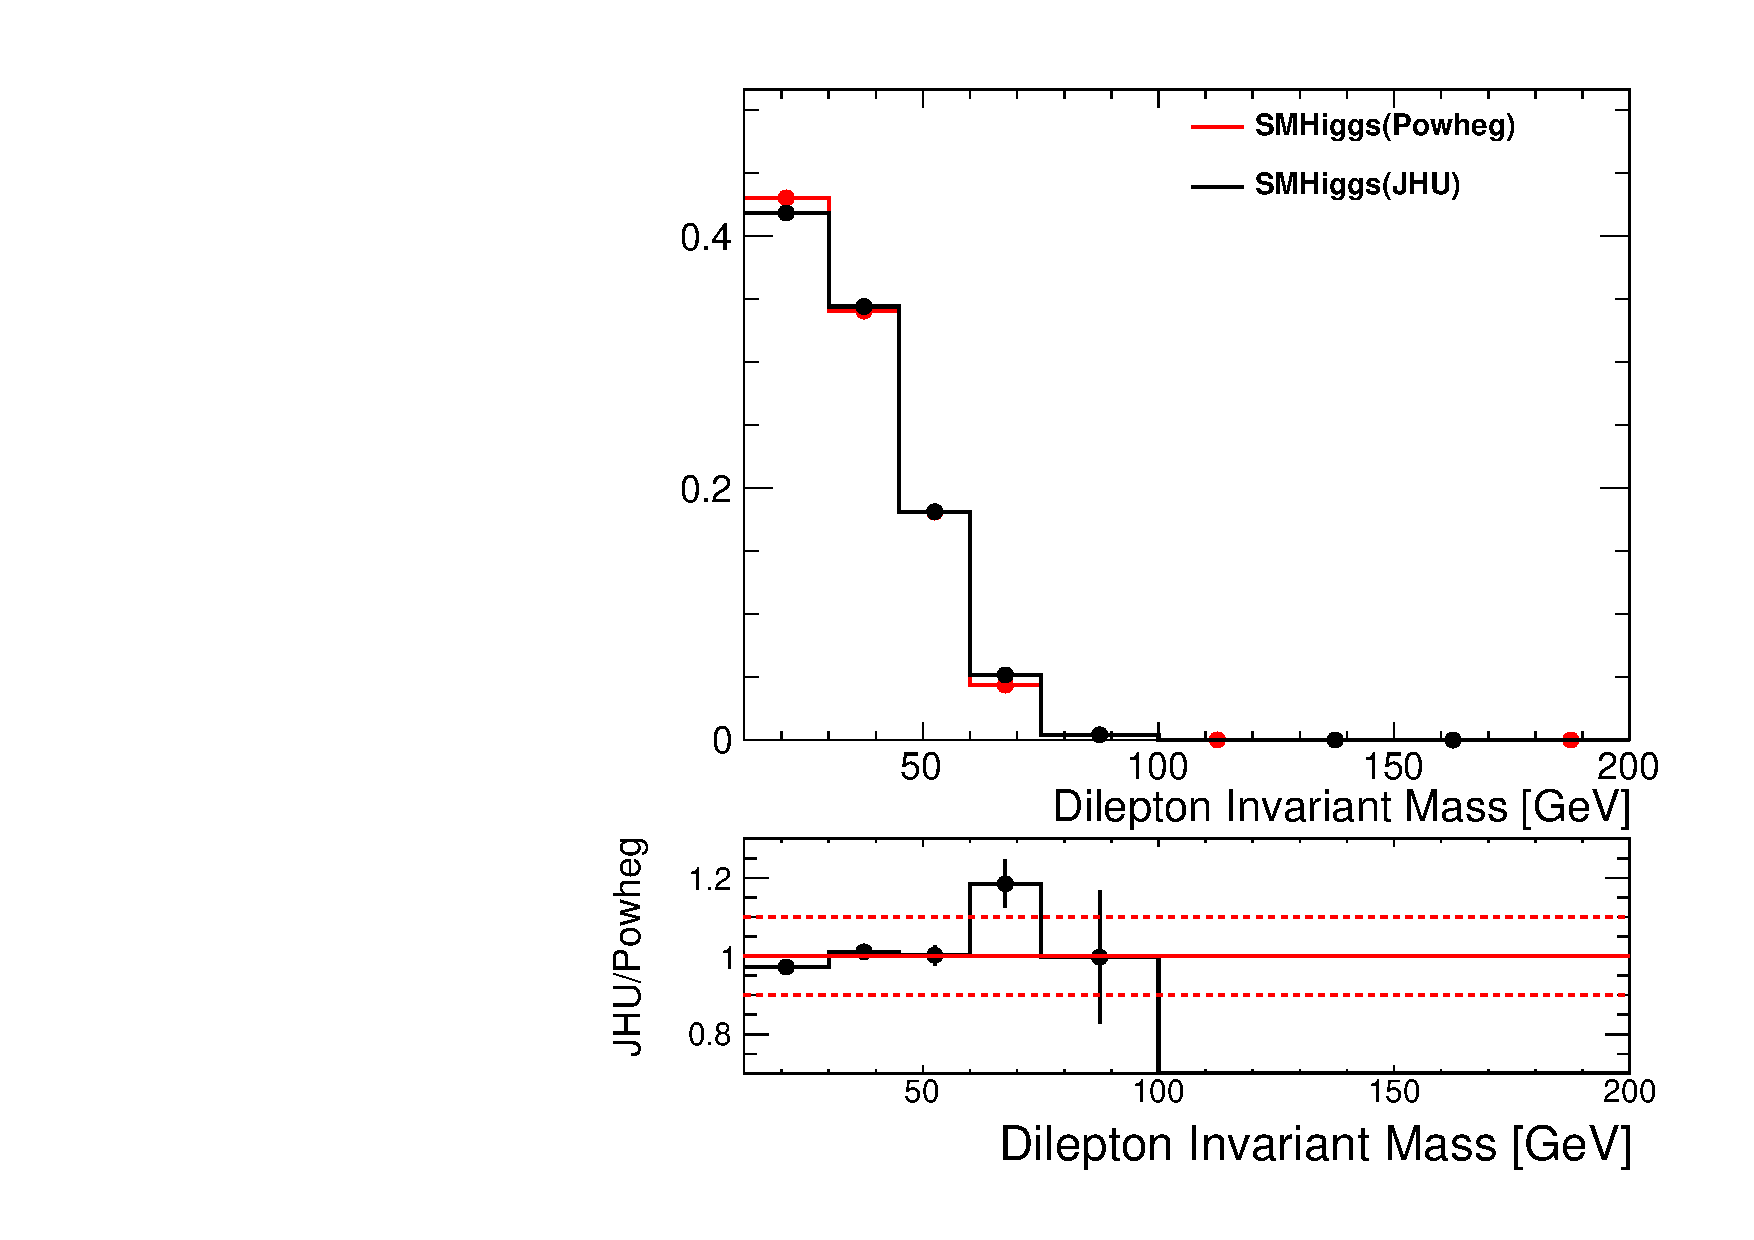
\includegraphics[width=.3\textwidth]{figures/mll.pdf}
} 
\subfigure[Transverse Higgs Mass]{
\centering
\label{subfig:mt}
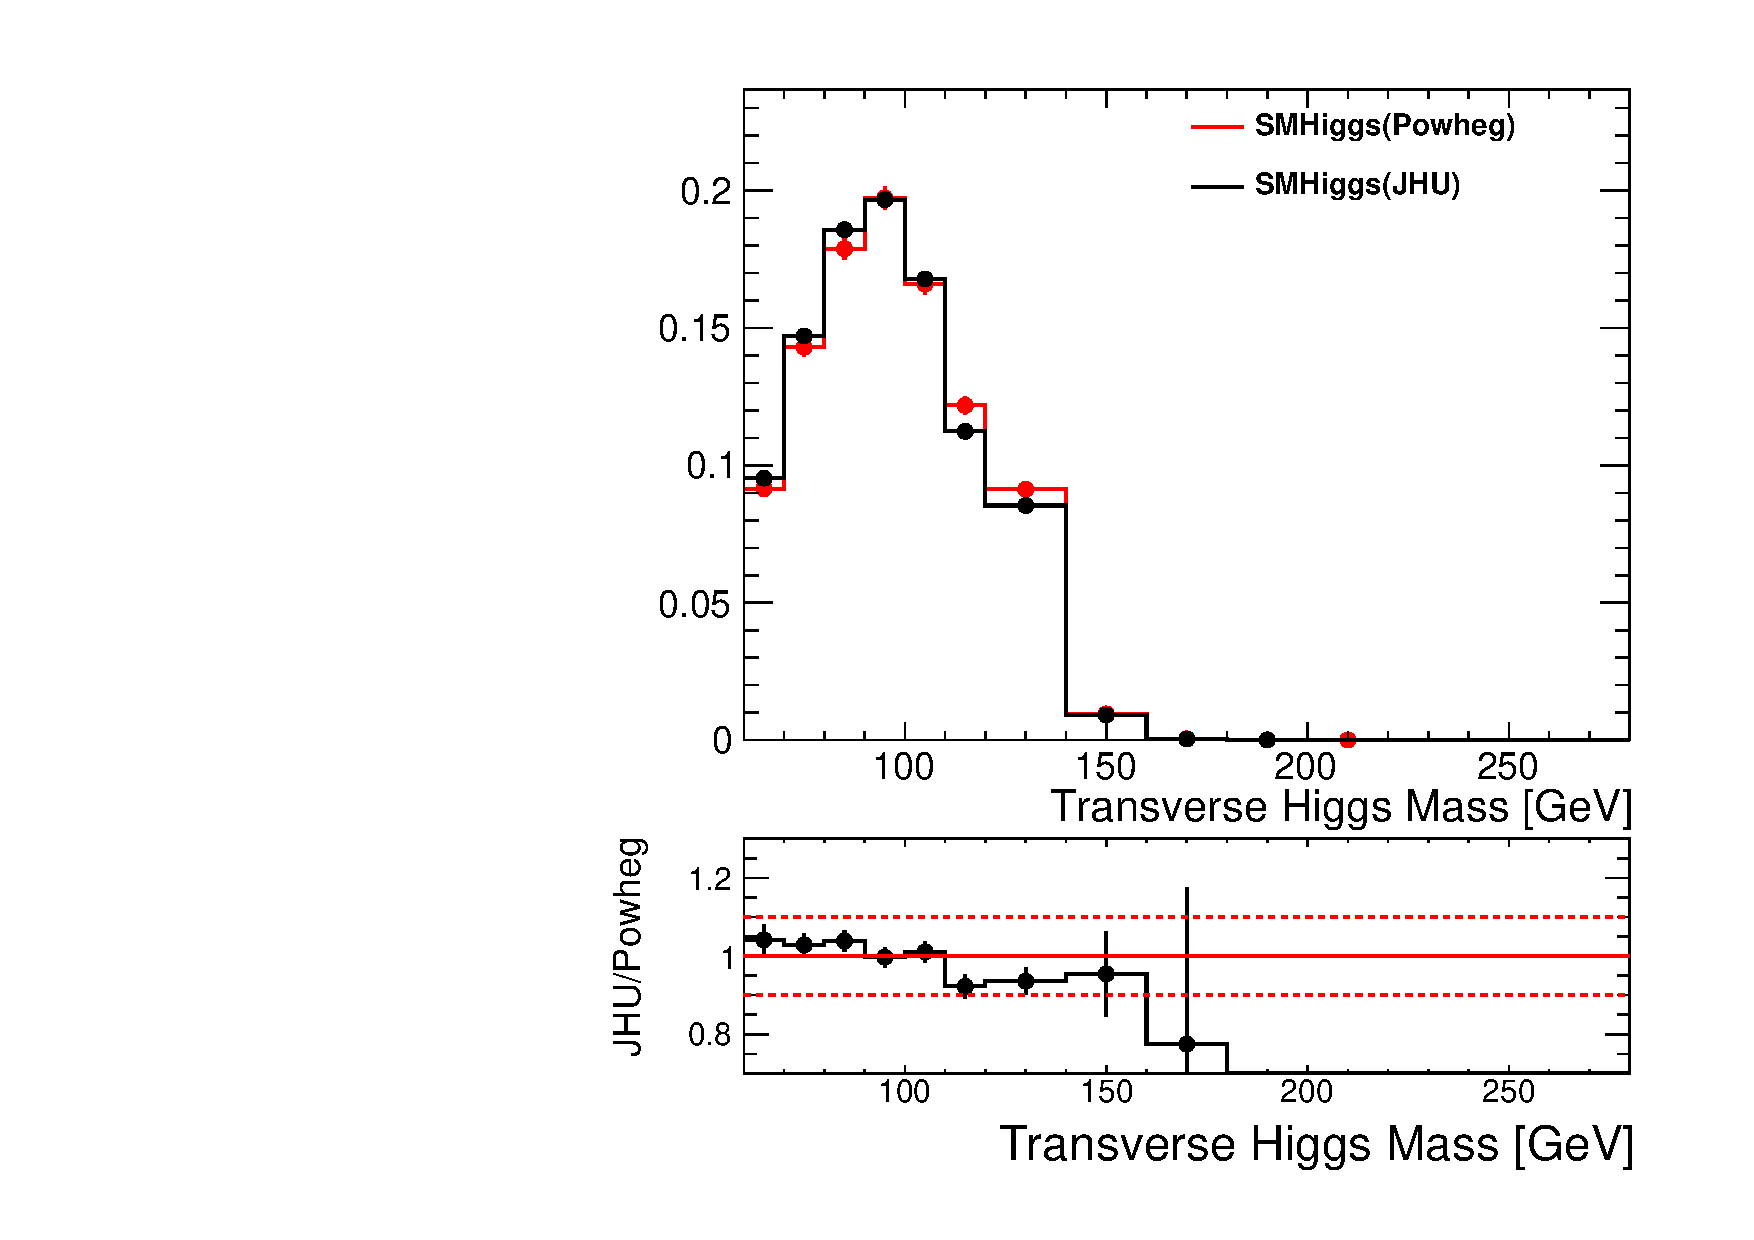
\includegraphics[width=.3\textwidth]{figures/mt.pdf}
}\\
\subfigure[Dilepton $\pt$]{
\centering
\label{subfig:dilpt}
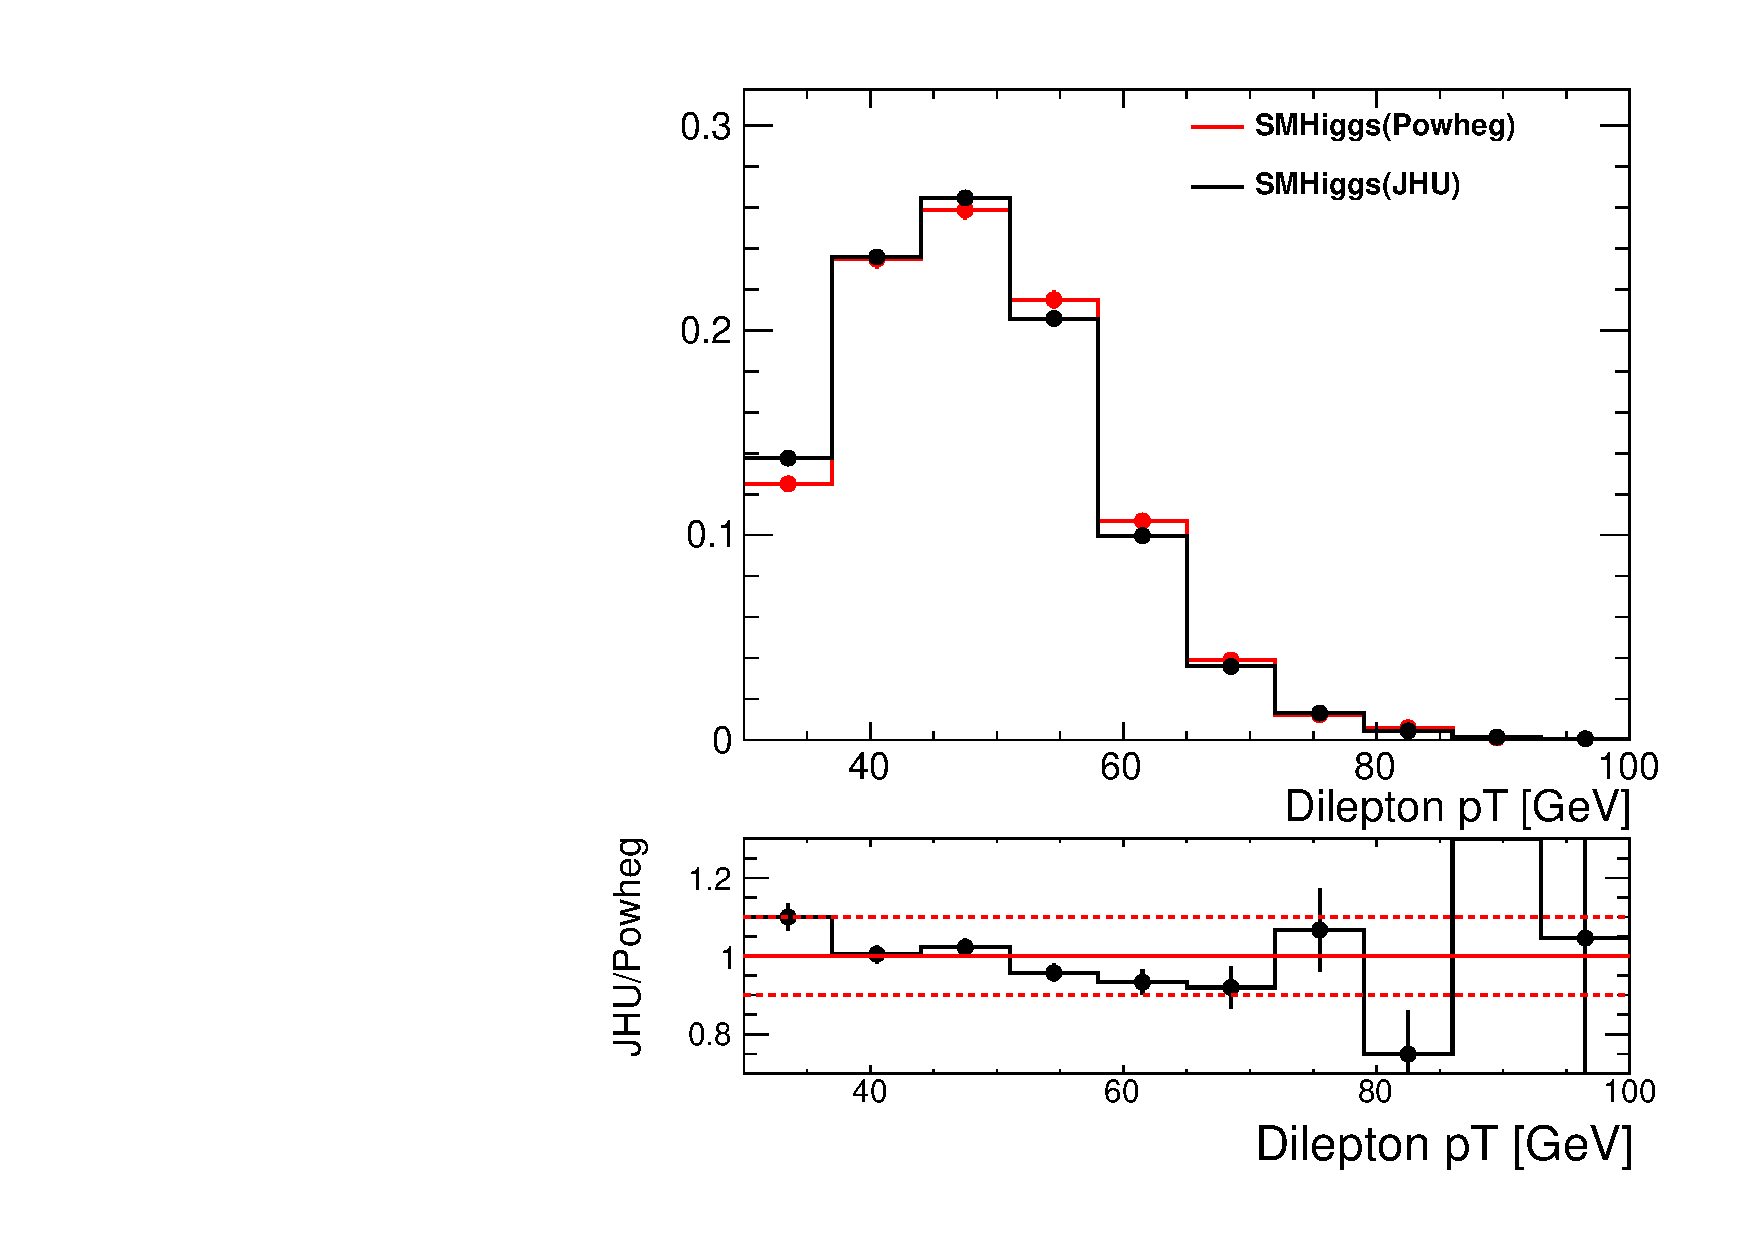
\includegraphics[width=.3\textwidth]{figures/dilpt.pdf}
}
\subfigure[Missing Energy]{
\centering
\label{subfig:met}
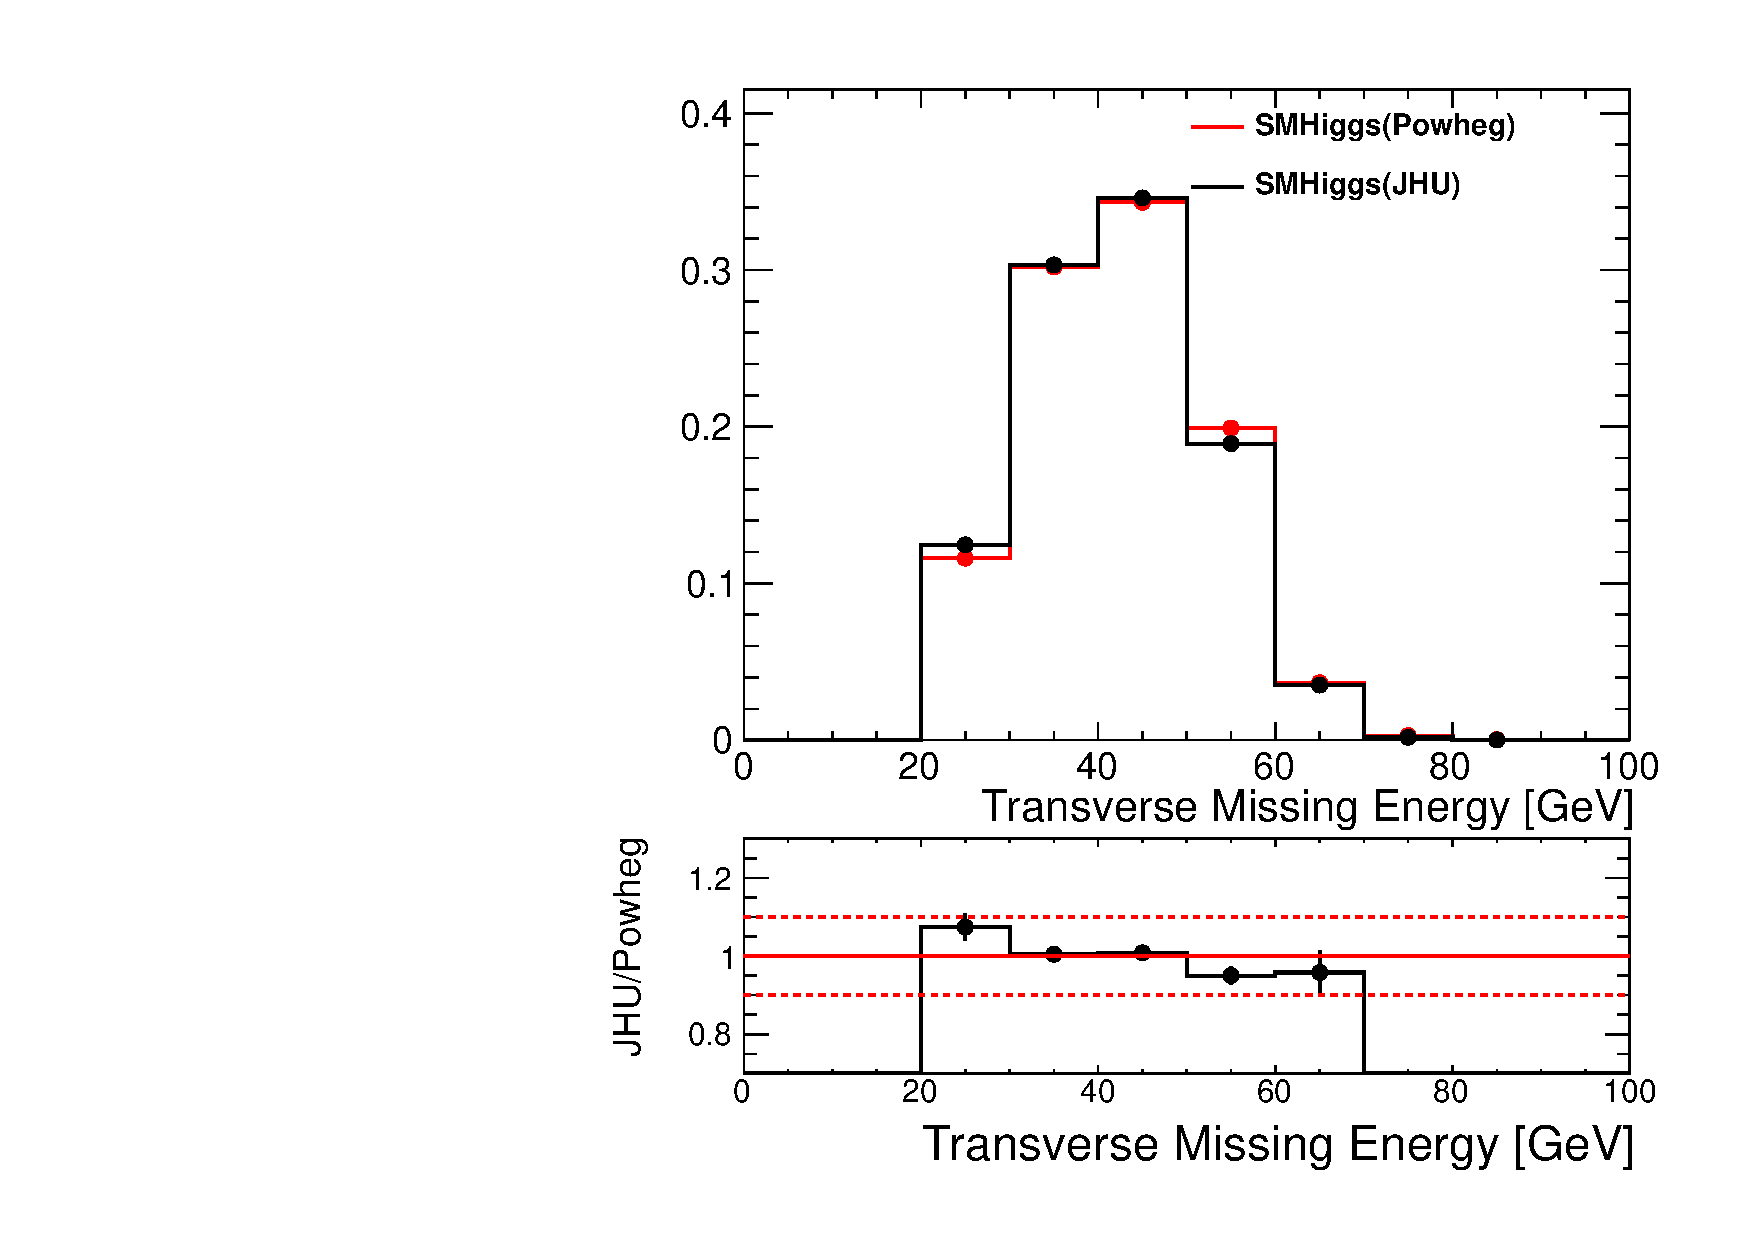
\includegraphics[width=.3\textwidth]{figures/met.pdf}
}
\subfigure[$\Delta\phi_{\ell\ell}$]{
\centering
\label{subfig:met}
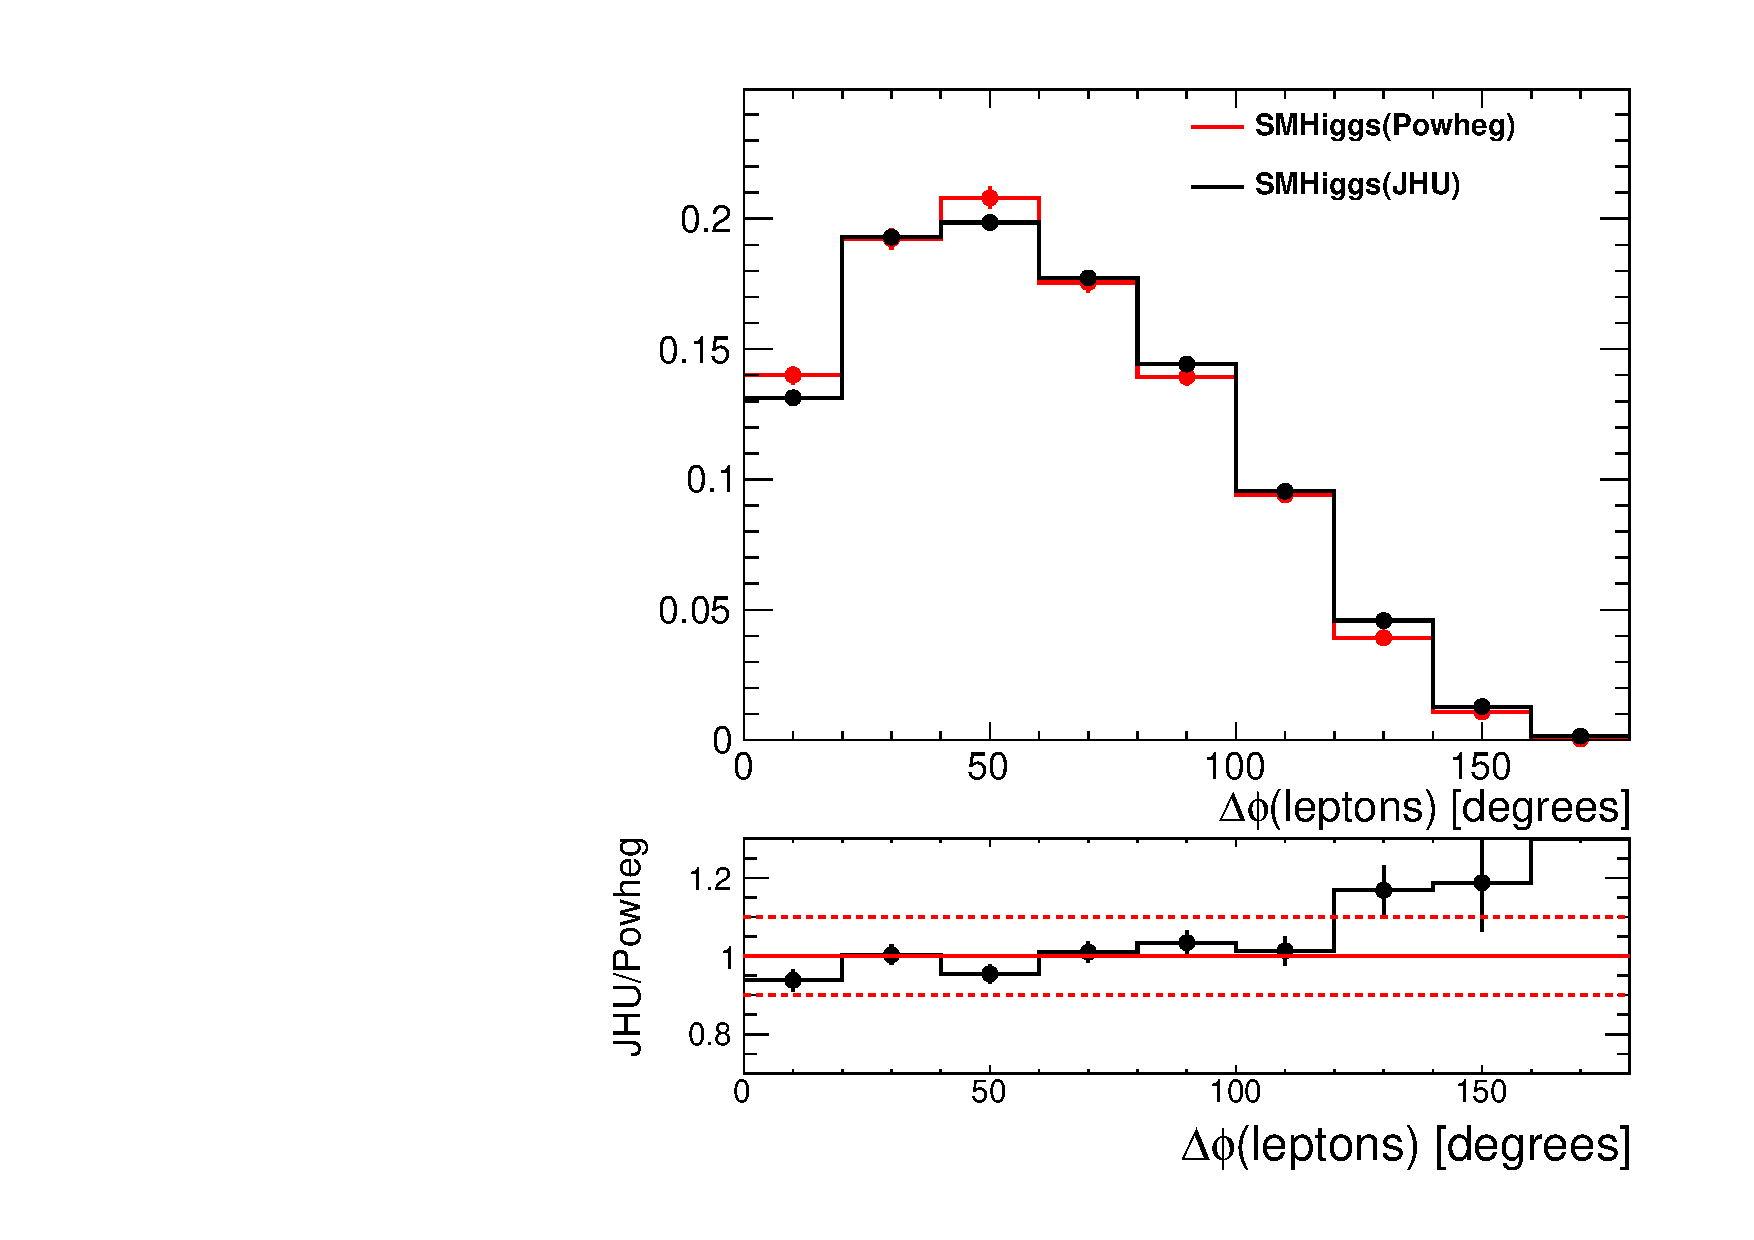
\includegraphics[width=.3\textwidth]{figures/dphill.pdf}
}\\
\caption{Kinematic distributions (normalized to 1) of the SM Higgs hypothesis 
comparing Powheg-Pythia and JHUGen-Pythia for reconstructed events 
after final event selections. }
\label{fig:higgskin_0j}
\end{figure}
%%%%%%%%%%%%%%%%%%%%%%%%%%%%%%%%%%%%%%%%%%%%%

%%%%%%%%%%%%%%%%%%%%%%%%%%%%%%%%%%%%%%%%%%%%%
\begin{figure}[!hbtp]
\centering
\subfigure[Higgs $\pt$]{
\centering
\label{subfig:higgspt_0j}
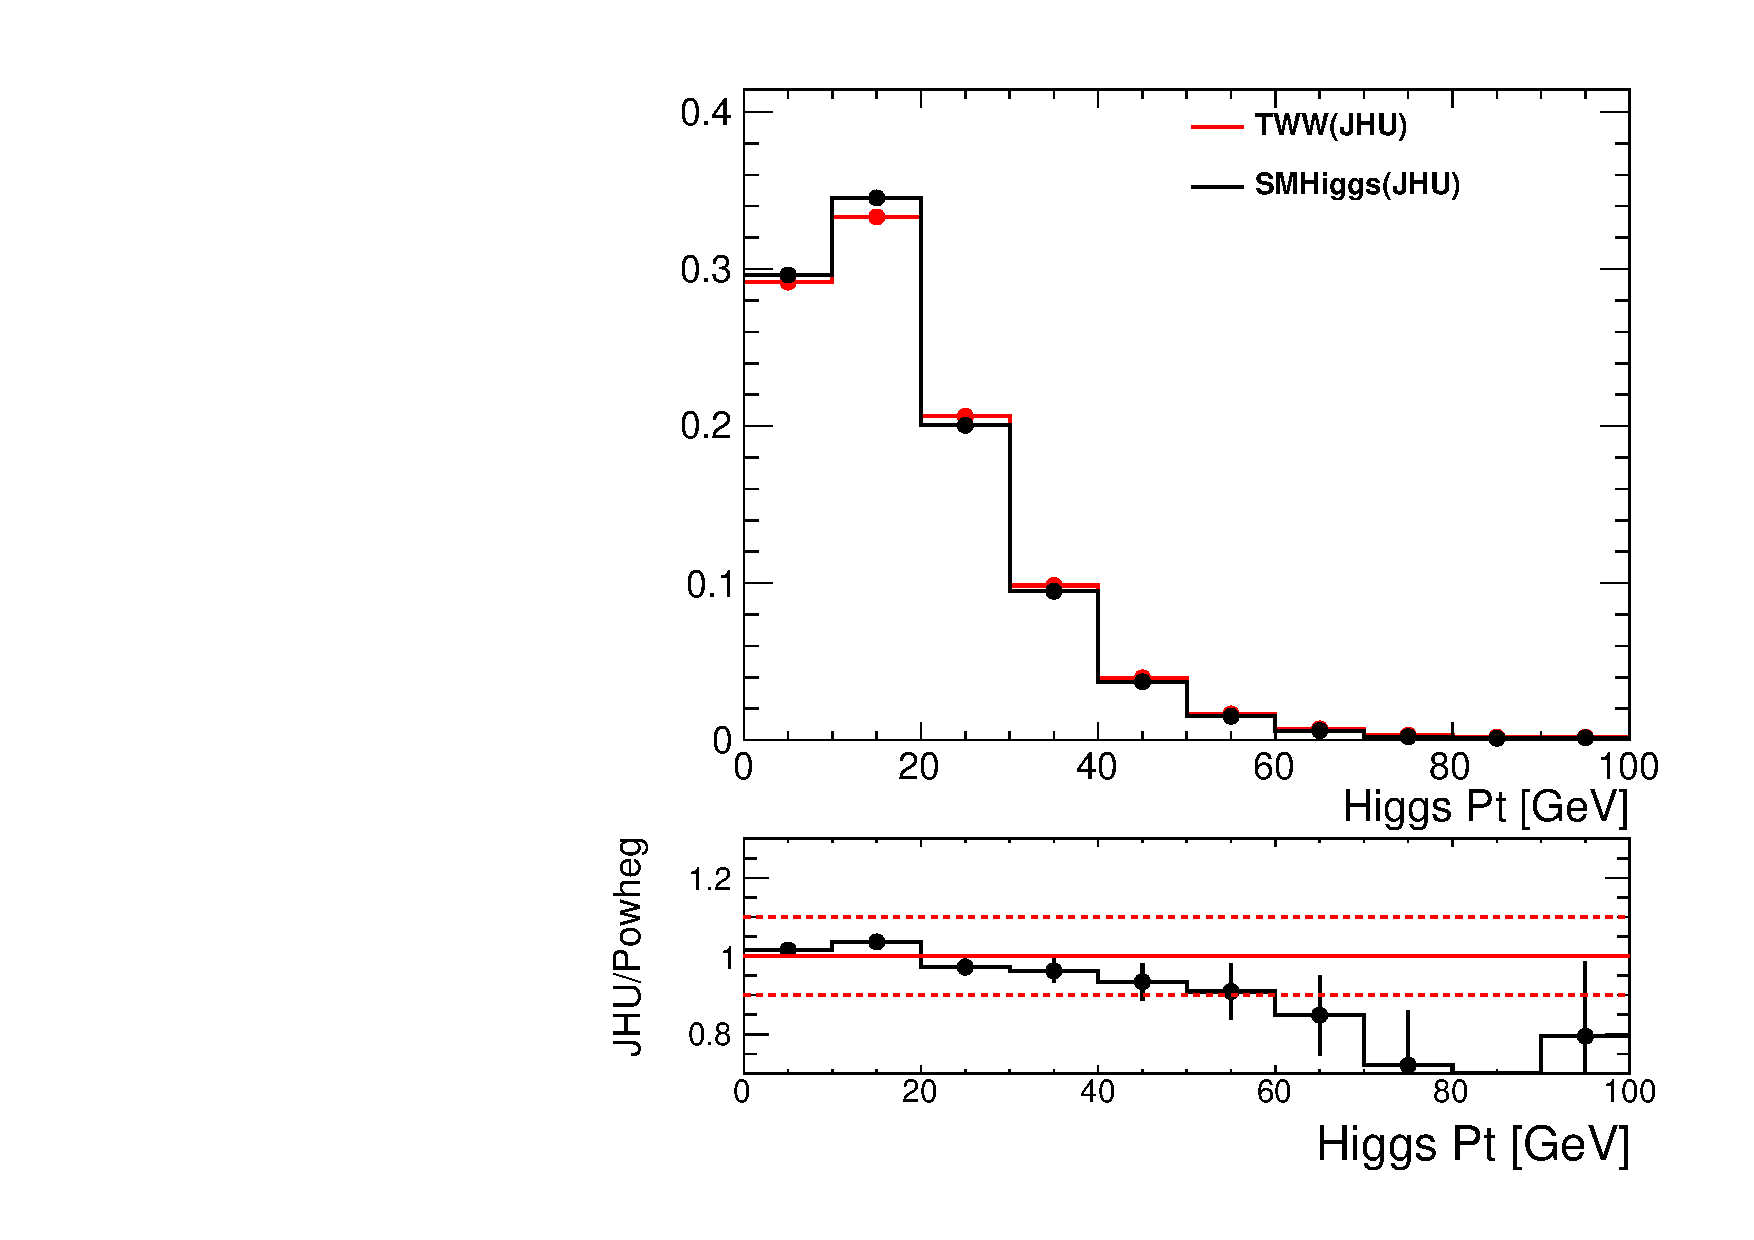
\includegraphics[width=.3\textwidth]{figures/higgsPt_gravitonvshiggs.pdf}
}
\subfigure[Leading Jet $\pt$]{
\centering
\label{subfig:jet1pt_0j}
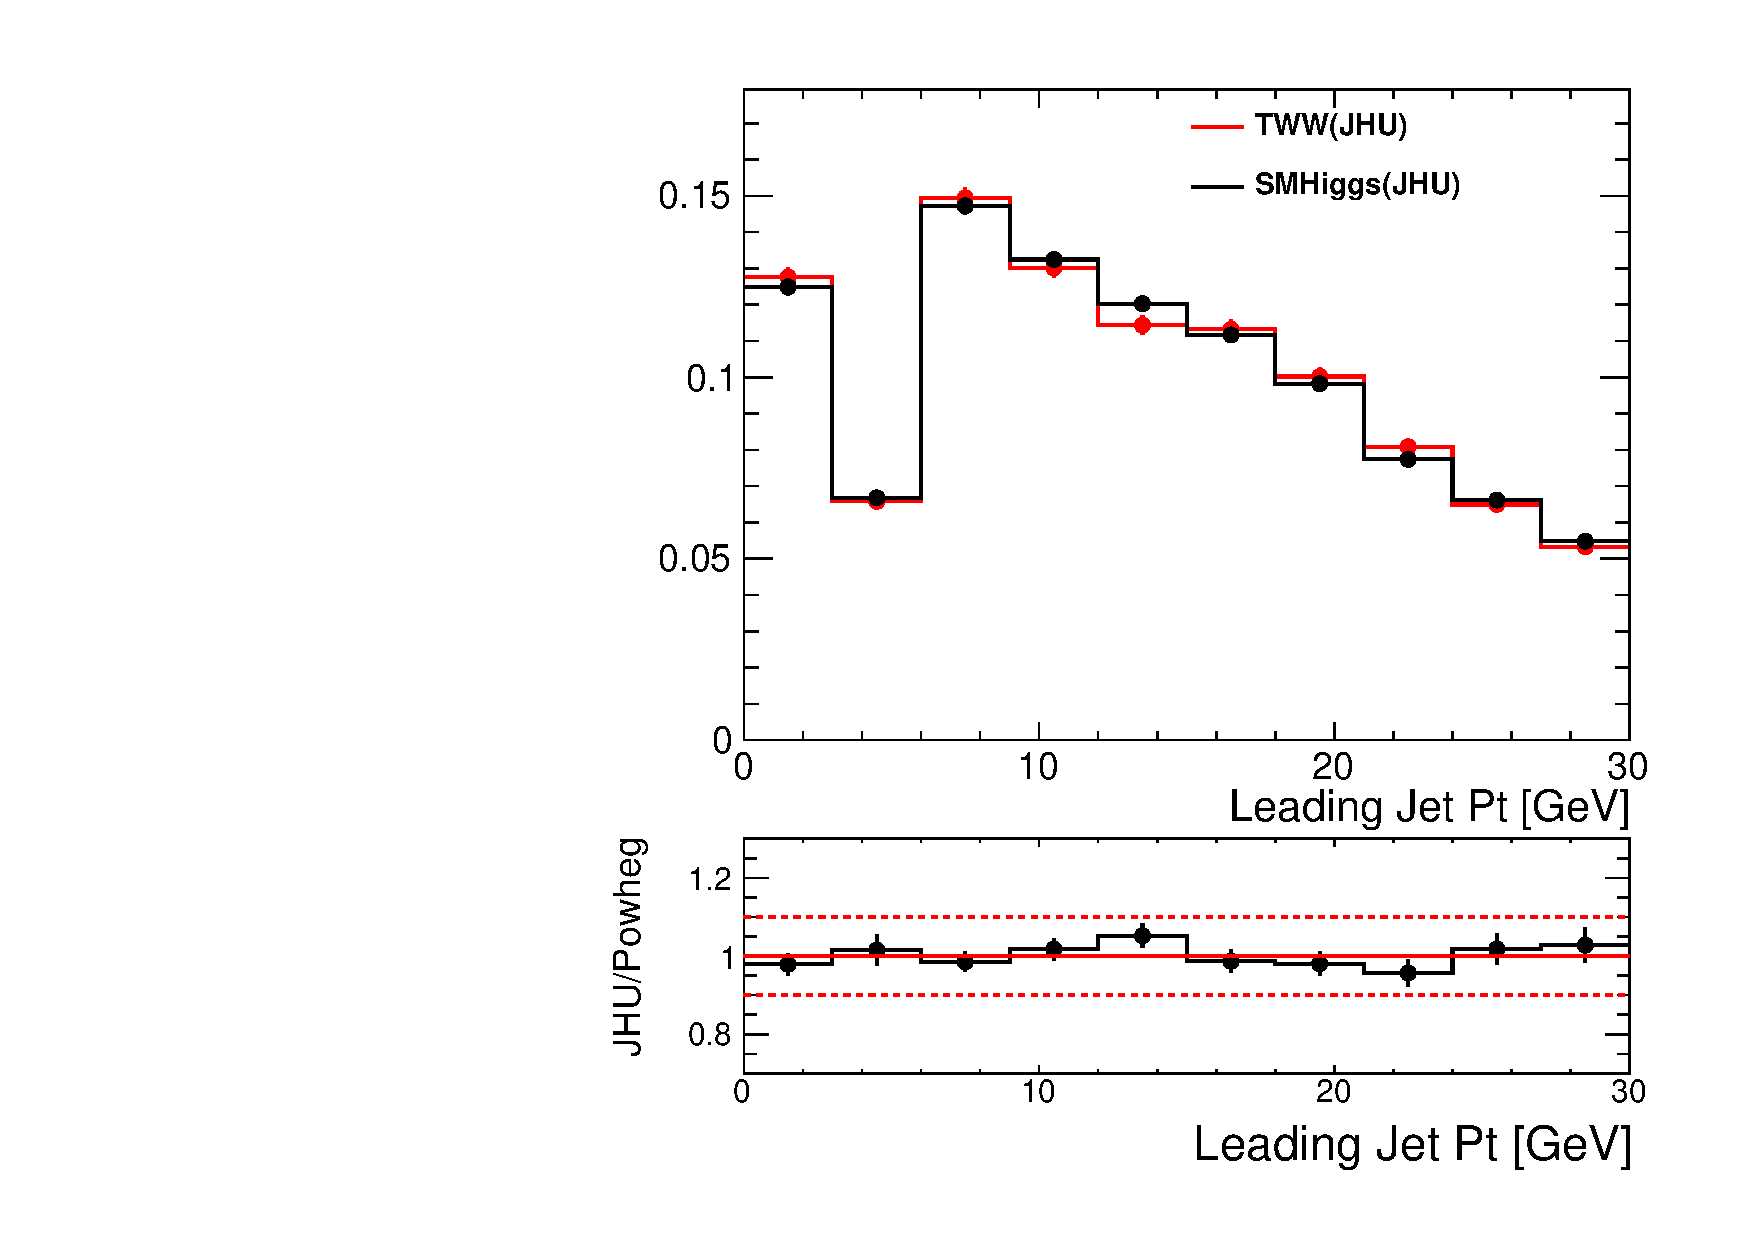
\includegraphics[width=.3\textwidth]{figures/jet1pt_gravitonvshiggs.pdf}
}\\
\caption{The Higgs $\pt$ and the leading jet $\pt$ distributions (normalized to 1) of the 
SM Higgs hypothesis compared to the Graviton ($2_\text{min}^+$) hypothesis, applying 
final event selections. }
\label{fig:gravvshiggspt_0j}
\end{figure}
%%%%%%%%%%%%%%%%%%%%%%%%%%%%%%%%%%%%%%%%%%%%%

